\documentclass[a4paper]{book}
\usepackage{makeidx}
\usepackage{natbib}
\usepackage{graphicx}
\usepackage{multicol}
\usepackage{float}
\usepackage{listings}
\usepackage{color}
\usepackage{ifthen}
\usepackage[table]{xcolor}
\usepackage{textcomp}
\usepackage{alltt}
\usepackage{ifpdf}
\ifpdf
\usepackage[pdftex,
            pagebackref=true,
            colorlinks=true,
            linkcolor=blue,
            unicode
           ]{hyperref}
\else
\usepackage[ps2pdf,
            pagebackref=true,
            colorlinks=true,
            linkcolor=blue,
            unicode
           ]{hyperref}
\usepackage{pspicture}
\fi
\usepackage[utf8]{inputenc}
Portuguese
\usepackage{mathptmx}
\usepackage[scaled=.90]{helvet}
\usepackage{courier}
\usepackage{sectsty}
\usepackage[titles]{tocloft}
\usepackage{doxygen}
\lstset{language=C++,inputencoding=utf8,basicstyle=\footnotesize,breaklines=true,breakatwhitespace=true,tabsize=8,numbers=left }
\makeindex
\setcounter{tocdepth}{3}
\renewcommand{\footrulewidth}{0.4pt}
\renewcommand{\familydefault}{\sfdefault}
\hfuzz=15pt
\setlength{\emergencystretch}{15pt}
\hbadness=750
\tolerance=750
\begin{document}
\hypersetup{pageanchor=false,citecolor=blue}
\begin{titlepage}
\vspace*{7cm}
\begin{center}
{\Large \-L\-Z5 \\[1ex]\large lz5\-\_\-turbo }\\
\vspace*{1cm}
{\large \-Gerado por Doxygen 1.7.6.1}\\
\vspace*{0.5cm}
{\small Terça, 29 de Janeiro de 2013 13:14:04}\\
\end{center}
\end{titlepage}
\clearemptydoublepage
\pagenumbering{roman}
\tableofcontents
\clearemptydoublepage
\pagenumbering{arabic}
\hypersetup{pageanchor=true,citecolor=blue}
\chapter{Índice dos componentes}
\section{\-Hierarquia de classes}
\-Esta lista de heranças está organizada, dentro do possível, por ordem alfabética\-:\begin{DoxyCompactList}
\item \contentsline{section}{\-Alelo}{\pageref{class_alelo}}{}
\begin{DoxyCompactList}
\item \contentsline{section}{\-Alelo\-Id}{\pageref{class_alelo_id}}{}
\end{DoxyCompactList}
\item \contentsline{section}{\-Geracao}{\pageref{class_geracao}}{}
\item \contentsline{section}{\-Individuo}{\pageref{class_individuo}}{}
\item \contentsline{section}{\-Loco}{\pageref{class_loco}}{}
\item \contentsline{section}{\-Populacao}{\pageref{class_populacao}}{}
\end{DoxyCompactList}

\chapter{Índice dos componentes}
\section{\-Lista de componentes}
\-Lista de classes, estruturas, uniões e interfaces com uma breve descrição\-:\begin{DoxyCompactList}
\item\contentsline{section}{\hyperlink{class_alelo}{\-Alelo} \\*\-Classe para criar um \hyperlink{class_alelo}{\-Alelo} }{\pageref{class_alelo}}{}
\item\contentsline{section}{\hyperlink{class_alelo_id}{\-Alelo\-Id} \\*\-Classe derivada para criar um \hyperlink{class_alelo}{\-Alelo} com sua identificacao (\-I\-D) }{\pageref{class_alelo_id}}{}
\item\contentsline{section}{\hyperlink{class_geracao}{\-Geracao} \\*\-Cria uma \hyperlink{class_geracao}{\-Geracao} que ira constituir uma populacao }{\pageref{class_geracao}}{}
\item\contentsline{section}{\hyperlink{class_individuo}{\-Individuo} \\*\-Cria um genoma que constitui um individuo }{\pageref{class_individuo}}{}
\item\contentsline{section}{\hyperlink{class_loco}{\-Loco} \\*\-Classe para criar um \hyperlink{class_loco}{\-Loco} a partir de 2 \-Alelos }{\pageref{class_loco}}{}
\item\contentsline{section}{\hyperlink{class_populacao}{\-Populacao} \\*\-Cria uma \hyperlink{class_populacao}{\-Populacao}, constituida de diversas \-Geracoes }{\pageref{class_populacao}}{}
\end{DoxyCompactList}

\chapter{Índice dos ficheiros}
\section{\-Lista de ficheiros}
\-Lista de todos os ficheiros com uma breve descrição\-:\begin{DoxyCompactList}
\item\contentsline{section}{/home/michel/workspace/\-L\-Z5/\hyperlink{alelo_8cpp}{alelo.\-cpp} }{\pageref{alelo_8cpp}}{}
\item\contentsline{section}{/home/michel/workspace/\-L\-Z5/\hyperlink{alelo_8h}{alelo.\-h} }{\pageref{alelo_8h}}{}
\item\contentsline{section}{/home/michel/workspace/\-L\-Z5/\hyperlink{geracao_8cpp}{geracao.\-cpp} }{\pageref{geracao_8cpp}}{}
\item\contentsline{section}{/home/michel/workspace/\-L\-Z5/\hyperlink{geracao_8h}{geracao.\-h} }{\pageref{geracao_8h}}{}
\item\contentsline{section}{/home/michel/workspace/\-L\-Z5/\hyperlink{individuo_8cpp}{individuo.\-cpp} }{\pageref{individuo_8cpp}}{}
\item\contentsline{section}{/home/michel/workspace/\-L\-Z5/\hyperlink{individuo_8h}{individuo.\-h} }{\pageref{individuo_8h}}{}
\item\contentsline{section}{/home/michel/workspace/\-L\-Z5/\hyperlink{loco_8cpp}{loco.\-cpp} }{\pageref{loco_8cpp}}{}
\item\contentsline{section}{/home/michel/workspace/\-L\-Z5/\hyperlink{loco_8h}{loco.\-h} }{\pageref{loco_8h}}{}
\item\contentsline{section}{/home/michel/workspace/\-L\-Z5/\hyperlink{lz5_8cpp}{lz5.\-cpp} }{\pageref{lz5_8cpp}}{}
\item\contentsline{section}{/home/michel/workspace/\-L\-Z5/\hyperlink{populacao_8cpp}{populacao.\-cpp} }{\pageref{populacao_8cpp}}{}
\item\contentsline{section}{/home/michel/workspace/\-L\-Z5/\hyperlink{populacao_8h}{populacao.\-h} }{\pageref{populacao_8h}}{}
\end{DoxyCompactList}

\chapter{\-Documentação da classe}
\hypertarget{class_alelo}{\section{\-Referência à classe \-Alelo}
\label{class_alelo}\index{\-Alelo@{\-Alelo}}
}


\-Classe para criar um \hyperlink{class_alelo}{\-Alelo}.  




{\ttfamily \#include $<$alelo.\-h$>$}



\-Diagrama de heranças da classe \-Alelo\nopagebreak
\begin{figure}[H]
\begin{center}
\leavevmode
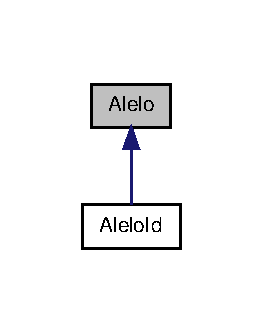
\includegraphics[width=126pt]{class_alelo__inherit__graph}
\end{center}
\end{figure}
\subsection*{\-Membros públicos}
\begin{DoxyCompactItemize}
\item 
\hyperlink{class_alelo_ab6a90be65041317c92a8976f4171cf62}{\-Alelo} ()
\item 
void \hyperlink{class_alelo_af01729982dc5849d6a6471383a30d918}{set\-Alelo} ()
\item 
bool \hyperlink{class_alelo_ace28885d23438e74674c3a7d68f5ea26}{get\-Alelo} ()
\end{DoxyCompactItemize}


\subsection{\-Descrição detalhada}
\-Classe para criar um \hyperlink{class_alelo}{\-Alelo}. 

\-A classe \hyperlink{class_alelo}{\-Alelo} tem como funcao representar um alelo na forma mais simples, podendo ser 0 ou 1, esta classe apenas representa o estado do alelo, sem armazenar valores ou efeitos para este. \-Esta eh uma classe base e, dependendo do tipo de simulacao pode-\/se usar a classe derivada \hyperlink{class_alelo_id}{\-Alelo\-Id}. \begin{DoxyAuthor}{\-Autor}
\-Michel \-Marques \-Farah e \-Ricardo da \-Fonseca 
\end{DoxyAuthor}
\begin{DoxySince}{\-Desde}
20/09/2012 
\end{DoxySince}
\begin{DoxyVersion}{\-Versão}
1.\-0 
\end{DoxyVersion}


\subsection{\-Documentação dos \-Construtores \& \-Destrutor}
\hypertarget{class_alelo_ab6a90be65041317c92a8976f4171cf62}{\index{\-Alelo@{\-Alelo}!\-Alelo@{\-Alelo}}
\index{\-Alelo@{\-Alelo}!Alelo@{\-Alelo}}
\subsubsection[{\-Alelo}]{\setlength{\rightskip}{0pt plus 5cm}{\bf \-Alelo\-::\-Alelo} (
\begin{DoxyParamCaption}
{}
\end{DoxyParamCaption}
)\hspace{0.3cm}{\ttfamily  \mbox{[}inline\mbox{]}}}}\label{class_alelo_ab6a90be65041317c92a8976f4171cf62}
armazena o estado do alelo, um valor bool indicando apenas se é \-F\-A\-L\-S\-E ou \-T\-R\-U\-E \-Por padrao o estado inicial do \hyperlink{class_alelo}{\-Alelo} sempre é \-F\-A\-L\-S\-E, sempre que chamado o metodo \hyperlink{class_alelo_af01729982dc5849d6a6471383a30d918}{set\-Alelo()} o estado do alelo se transforma para \-T\-R\-U\-E 

\subsection{\-Documentação dos métodos}
\hypertarget{class_alelo_ace28885d23438e74674c3a7d68f5ea26}{\index{\-Alelo@{\-Alelo}!get\-Alelo@{get\-Alelo}}
\index{get\-Alelo@{get\-Alelo}!Alelo@{\-Alelo}}
\subsubsection[{get\-Alelo}]{\setlength{\rightskip}{0pt plus 5cm}bool {\bf \-Alelo\-::get\-Alelo} (
\begin{DoxyParamCaption}
{}
\end{DoxyParamCaption}
)\hspace{0.3cm}{\ttfamily  \mbox{[}inline\mbox{]}}}}\label{class_alelo_ace28885d23438e74674c3a7d68f5ea26}
\-Retorna o estado atual do \hyperlink{class_alelo}{\-Alelo} \hypertarget{class_alelo_af01729982dc5849d6a6471383a30d918}{\index{\-Alelo@{\-Alelo}!set\-Alelo@{set\-Alelo}}
\index{set\-Alelo@{set\-Alelo}!Alelo@{\-Alelo}}
\subsubsection[{set\-Alelo}]{\setlength{\rightskip}{0pt plus 5cm}void {\bf \-Alelo\-::set\-Alelo} (
\begin{DoxyParamCaption}
{}
\end{DoxyParamCaption}
)\hspace{0.3cm}{\ttfamily  \mbox{[}inline\mbox{]}}}}\label{class_alelo_af01729982dc5849d6a6471383a30d918}
\-Altera o estado do \hyperlink{class_alelo}{\-Alelo} de \-F\-A\-L\-S\-E para \-T\-R\-U\-E 

\-A documentação para esta classe foi gerada a partir do seguinte ficheiro\-:\begin{DoxyCompactItemize}
\item 
/home/michel/workspace/\-L\-Z5/\hyperlink{alelo_8h}{alelo.\-h}\end{DoxyCompactItemize}

\hypertarget{class_alelo_id}{\section{\-Referência à classe \-Alelo\-Id}
\label{class_alelo_id}\index{\-Alelo\-Id@{\-Alelo\-Id}}
}


\-Classe derivada para criar um \hyperlink{class_alelo}{\-Alelo} com sua identificacao (\-I\-D).  




{\ttfamily \#include $<$alelo.\-h$>$}



\-Diagrama de heranças da classe \-Alelo\-Id\nopagebreak
\begin{figure}[H]
\begin{center}
\leavevmode
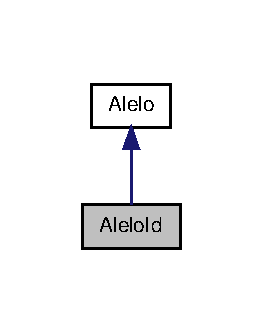
\includegraphics[width=126pt]{class_alelo_id__inherit__graph}
\end{center}
\end{figure}


\-Diagrama de colaboração para \-Alelo\-Id\-:\nopagebreak
\begin{figure}[H]
\begin{center}
\leavevmode
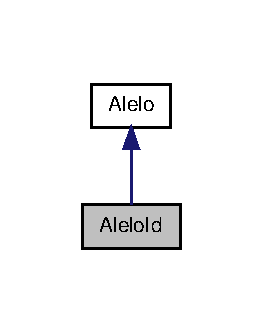
\includegraphics[width=126pt]{class_alelo_id__coll__graph}
\end{center}
\end{figure}
\subsection*{\-Membros públicos}
\begin{DoxyCompactItemize}
\item 
\hyperlink{class_alelo_id_ad7a7d64a5cfd3c7bbc44d81f3d5b4380}{\-Alelo\-Id} ()
\item 
unsigned int \hyperlink{class_alelo_id_ab825afe5e781e2e072009b104d0ef4e7}{get\-Id} ()
\end{DoxyCompactItemize}


\subsection{\-Descrição detalhada}
\-Classe derivada para criar um \hyperlink{class_alelo}{\-Alelo} com sua identificacao (\-I\-D). 

\-A classe \hyperlink{class_alelo_id}{\-Alelo\-Id} eh uma classe derivada da \hyperlink{class_alelo}{\-Alelo} e tem como finalidade criar um alelo marcador com identificao para estudos que envolvem o conceito de locos identicos por descendencia (ibd). \-Assim, quando desejado, o simulador cria uma identificacao unica para cada novo \hyperlink{class_alelo}{\-Alelo} criado. 

\subsection{\-Documentação dos \-Construtores \& \-Destrutor}
\hypertarget{class_alelo_id_ad7a7d64a5cfd3c7bbc44d81f3d5b4380}{\index{\-Alelo\-Id@{\-Alelo\-Id}!\-Alelo\-Id@{\-Alelo\-Id}}
\index{\-Alelo\-Id@{\-Alelo\-Id}!AleloId@{\-Alelo\-Id}}
\subsubsection[{\-Alelo\-Id}]{\setlength{\rightskip}{0pt plus 5cm}{\bf \-Alelo\-Id\-::\-Alelo\-Id} (
\begin{DoxyParamCaption}
{}
\end{DoxyParamCaption}
)\hspace{0.3cm}{\ttfamily  \mbox{[}inline\mbox{]}}}}\label{class_alelo_id_ad7a7d64a5cfd3c7bbc44d81f3d5b4380}
\-Apresenta a mesma configuracao da \-Clase \-Base \hyperlink{class_alelo}{\-Alelo}, porem, cada vez que um \hyperlink{class_alelo_id}{\-Alelo\-Id} eh criado ele armazena uma identificacao definida pelo contador 'cont'. 

\subsection{\-Documentação dos métodos}
\hypertarget{class_alelo_id_ab825afe5e781e2e072009b104d0ef4e7}{\index{\-Alelo\-Id@{\-Alelo\-Id}!get\-Id@{get\-Id}}
\index{get\-Id@{get\-Id}!AleloId@{\-Alelo\-Id}}
\subsubsection[{get\-Id}]{\setlength{\rightskip}{0pt plus 5cm}unsigned int {\bf \-Alelo\-Id\-::get\-Id} (
\begin{DoxyParamCaption}
{}
\end{DoxyParamCaption}
)\hspace{0.3cm}{\ttfamily  \mbox{[}inline\mbox{]}}}}\label{class_alelo_id_ab825afe5e781e2e072009b104d0ef4e7}
\-Retorna o \-I\-D do \hyperlink{class_alelo}{\-Alelo} 

\-A documentação para esta classe foi gerada a partir dos seguintes ficheiros\-:\begin{DoxyCompactItemize}
\item 
/home/michel/workspace/\-L\-Z5/\hyperlink{alelo_8h}{alelo.\-h}\item 
/home/michel/workspace/\-L\-Z5/\hyperlink{alelo_8cpp}{alelo.\-cpp}\end{DoxyCompactItemize}

\hypertarget{class_geracao}{\section{\-Referência à classe \-Geracao}
\label{class_geracao}\index{\-Geracao@{\-Geracao}}
}


\-Cria uma \hyperlink{class_geracao}{\-Geracao} que ira constituir uma populacao.  




{\ttfamily \#include $<$geracao.\-h$>$}

\subsection*{\-Membros públicos}
\begin{DoxyCompactItemize}
\item 
\hyperlink{class_geracao_a52622873ac80a7d688e827b7430f7fe1}{\-Geracao} ()
\item 
void \hyperlink{class_geracao_ad06d071bed257d62506aa47a5186496f}{set\-Geracao} (unsigned int tampb, bool tipo, float varres, float mediavarres, unsigned int qtdlocos, unsigned int qtdqtl, unsigned int qtdmarcador, float varad, float freqp, float freqpqtl, float pvaqtl, unsigned int qtdcrom)
\item 
void \hyperlink{class_geracao_affc43315799b830a85c176072c5607ae}{set\-Varadg} ()
\item 
void \hyperlink{class_geracao_a8b139af5fcd3e5c5b302720cd6cabea0}{set\-Varresg} ()
\item 
void \hyperlink{class_geracao_adc9964b180ec37ecf40ba517a88f2c55}{set\-Mediag} ()
\item 
int \hyperlink{class_geracao_a58da88c6b6153dffd868cce13cade519}{get\-Tam\-Ger} ()
\item 
vector$<$ \hyperlink{class_individuo}{\-Individuo} $\ast$ $>$ \hyperlink{class_geracao_a313a62ad95ce1050c172954966bb83dd}{get\-Geracao} ()
\item 
float \hyperlink{class_geracao_a26583f8146e5f3e17f599a29646cc308}{get\-Varadg} ()
\item 
float \hyperlink{class_geracao_abda536f06142339a57e0b44ec52c0af1}{get\-Varresg} ()
\item 
float \hyperlink{class_geracao_a3ba1a1b0f86c1639af46e68263aa09c2}{get\-Varfeng} ()
\item 
float \hyperlink{class_geracao_a236ba45bf2ebe94e5d535e9e98bfa6a7}{get\-Mediag} ()
\end{DoxyCompactItemize}


\subsection{\-Descrição detalhada}
\-Cria uma \hyperlink{class_geracao}{\-Geracao} que ira constituir uma populacao. 

\-A classe \hyperlink{class_geracao}{\-Geracao} aramazena um conjunto de \-Individuos contemporaneos. \-Esta classe tem como funcao facilitar o controle da simulacao por \hyperlink{class_geracao}{\-Geracao}, fornecendo paramentros populacionais para cada geracao criada. 

\subsection{\-Documentação dos \-Construtores \& \-Destrutor}
\hypertarget{class_geracao_a52622873ac80a7d688e827b7430f7fe1}{\index{\-Geracao@{\-Geracao}!\-Geracao@{\-Geracao}}
\index{\-Geracao@{\-Geracao}!Geracao@{\-Geracao}}
\subsubsection[{\-Geracao}]{\setlength{\rightskip}{0pt plus 5cm}{\bf \-Geracao\-::\-Geracao} (
\begin{DoxyParamCaption}
{}
\end{DoxyParamCaption}
)\hspace{0.3cm}{\ttfamily  \mbox{[}inline\mbox{]}}}}\label{class_geracao_a52622873ac80a7d688e827b7430f7fe1}
\-Armazena a media da caracteristica na geracao. 

\subsection{\-Documentação dos métodos}
\hypertarget{class_geracao_a313a62ad95ce1050c172954966bb83dd}{\index{\-Geracao@{\-Geracao}!get\-Geracao@{get\-Geracao}}
\index{get\-Geracao@{get\-Geracao}!Geracao@{\-Geracao}}
\subsubsection[{get\-Geracao}]{\setlength{\rightskip}{0pt plus 5cm}vector$<${\bf \-Individuo}$\ast$$>$ {\bf \-Geracao\-::get\-Geracao} (
\begin{DoxyParamCaption}
{}
\end{DoxyParamCaption}
)\hspace{0.3cm}{\ttfamily  \mbox{[}inline\mbox{]}}}}\label{class_geracao_a313a62ad95ce1050c172954966bb83dd}
\-Retorna o vetor de individuo da geracao. \hypertarget{class_geracao_a236ba45bf2ebe94e5d535e9e98bfa6a7}{\index{\-Geracao@{\-Geracao}!get\-Mediag@{get\-Mediag}}
\index{get\-Mediag@{get\-Mediag}!Geracao@{\-Geracao}}
\subsubsection[{get\-Mediag}]{\setlength{\rightskip}{0pt plus 5cm}float {\bf \-Geracao\-::get\-Mediag} (
\begin{DoxyParamCaption}
{}
\end{DoxyParamCaption}
)\hspace{0.3cm}{\ttfamily  \mbox{[}inline\mbox{]}}}}\label{class_geracao_a236ba45bf2ebe94e5d535e9e98bfa6a7}
\-Retorna a media da caracterista na geracao \hypertarget{class_geracao_a58da88c6b6153dffd868cce13cade519}{\index{\-Geracao@{\-Geracao}!get\-Tam\-Ger@{get\-Tam\-Ger}}
\index{get\-Tam\-Ger@{get\-Tam\-Ger}!Geracao@{\-Geracao}}
\subsubsection[{get\-Tam\-Ger}]{\setlength{\rightskip}{0pt plus 5cm}int {\bf \-Geracao\-::get\-Tam\-Ger} (
\begin{DoxyParamCaption}
{}
\end{DoxyParamCaption}
)\hspace{0.3cm}{\ttfamily  \mbox{[}inline\mbox{]}}}}\label{class_geracao_a58da88c6b6153dffd868cce13cade519}
\-Retorna o numero de individuos que constitui a geracao. \hypertarget{class_geracao_a26583f8146e5f3e17f599a29646cc308}{\index{\-Geracao@{\-Geracao}!get\-Varadg@{get\-Varadg}}
\index{get\-Varadg@{get\-Varadg}!Geracao@{\-Geracao}}
\subsubsection[{get\-Varadg}]{\setlength{\rightskip}{0pt plus 5cm}float {\bf \-Geracao\-::get\-Varadg} (
\begin{DoxyParamCaption}
{}
\end{DoxyParamCaption}
)\hspace{0.3cm}{\ttfamily  \mbox{[}inline\mbox{]}}}}\label{class_geracao_a26583f8146e5f3e17f599a29646cc308}
\-Retorna a variancia genetica aditiva da geracao 

\-Este é o diagrama das funções que utilizam esta função\-:\nopagebreak
\begin{figure}[H]
\begin{center}
\leavevmode
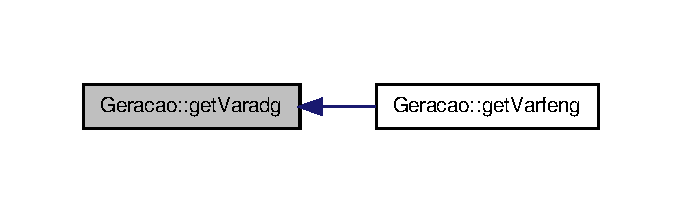
\includegraphics[width=328pt]{class_geracao_a26583f8146e5f3e17f599a29646cc308_icgraph}
\end{center}
\end{figure}


\hypertarget{class_geracao_a3ba1a1b0f86c1639af46e68263aa09c2}{\index{\-Geracao@{\-Geracao}!get\-Varfeng@{get\-Varfeng}}
\index{get\-Varfeng@{get\-Varfeng}!Geracao@{\-Geracao}}
\subsubsection[{get\-Varfeng}]{\setlength{\rightskip}{0pt plus 5cm}float {\bf \-Geracao\-::get\-Varfeng} (
\begin{DoxyParamCaption}
{}
\end{DoxyParamCaption}
)\hspace{0.3cm}{\ttfamily  \mbox{[}inline\mbox{]}}}}\label{class_geracao_a3ba1a1b0f86c1639af46e68263aa09c2}
\-Retorna a variancia fenotipica da geracao 

\-Grafo de chamadas desta função\-:\nopagebreak
\begin{figure}[H]
\begin{center}
\leavevmode
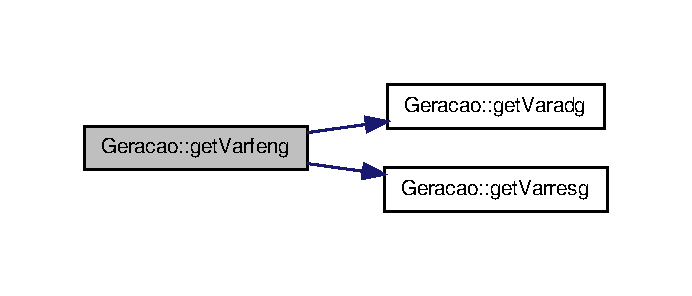
\includegraphics[width=332pt]{class_geracao_a3ba1a1b0f86c1639af46e68263aa09c2_cgraph}
\end{center}
\end{figure}


\hypertarget{class_geracao_abda536f06142339a57e0b44ec52c0af1}{\index{\-Geracao@{\-Geracao}!get\-Varresg@{get\-Varresg}}
\index{get\-Varresg@{get\-Varresg}!Geracao@{\-Geracao}}
\subsubsection[{get\-Varresg}]{\setlength{\rightskip}{0pt plus 5cm}float {\bf \-Geracao\-::get\-Varresg} (
\begin{DoxyParamCaption}
{}
\end{DoxyParamCaption}
)\hspace{0.3cm}{\ttfamily  \mbox{[}inline\mbox{]}}}}\label{class_geracao_abda536f06142339a57e0b44ec52c0af1}
\-Retorna a variancia residual da geracao 

\-Este é o diagrama das funções que utilizam esta função\-:\nopagebreak
\begin{figure}[H]
\begin{center}
\leavevmode
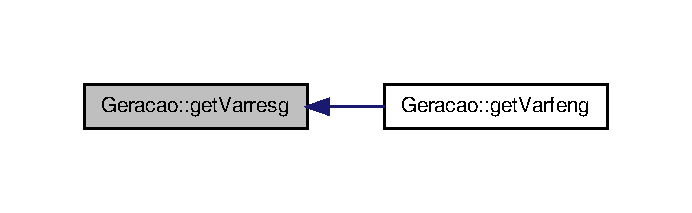
\includegraphics[width=332pt]{class_geracao_abda536f06142339a57e0b44ec52c0af1_icgraph}
\end{center}
\end{figure}


\hypertarget{class_geracao_ad06d071bed257d62506aa47a5186496f}{\index{\-Geracao@{\-Geracao}!set\-Geracao@{set\-Geracao}}
\index{set\-Geracao@{set\-Geracao}!Geracao@{\-Geracao}}
\subsubsection[{set\-Geracao}]{\setlength{\rightskip}{0pt plus 5cm}void {\bf \-Geracao\-::set\-Geracao} (
\begin{DoxyParamCaption}
\item[{unsigned int}]{tampb, }
\item[{bool}]{tipo, }
\item[{float}]{varres, }
\item[{float}]{mediavarres, }
\item[{unsigned int}]{qtdlocos, }
\item[{unsigned int}]{qtdqtl, }
\item[{unsigned int}]{qtdmarcador, }
\item[{float}]{varad, }
\item[{float}]{freqp, }
\item[{float}]{freqpqtl, }
\item[{float}]{pvaqtl, }
\item[{unsigned int}]{qtdcrom}
\end{DoxyParamCaption}
)}}\label{class_geracao_ad06d071bed257d62506aa47a5186496f}
\-Metodo para ajustar uma geracao. \-Se o contg for igual a zero, o simulador cria uma populacao base, ajustando todos os paramentros necessarios para realizar a simulacao (\hyperlink{class_individuo_ae89912e2bcf4391c30d6a5074f709c88}{\-Individuo\-::setpos\-T\-Locos()}, \hyperlink{class_individuo_a2366e00f66ed23bd142a1d63509098e4}{\-Individuo\-::set\-Tam\-Crom()}, \hyperlink{class_individuo_a93f10457d66068fe4e358a495d2e494c}{\-Individuo\-::criar\-Ind\-B()}). 
\begin{DoxyParams}{\-Parâmetros}
{\em tambp} & -\/ \-Tamanho da populacao base; \\
\hline
{\em tipo} & -\/ ver \hyperlink{class_loco_a17e42d11b5d0f86797f942742c476f04}{\-Loco\-::set\-Loco()}; \\
\hline
{\em varres} & -\/ \-Variancia \-Residual fornecida pelo usuario; \\
\hline
{\em mediavarres} & -\/ \-Media da variancia residual fornecida pelo usuario; \\
\hline
{\em qtdlocos} & -\/ \-Quantidade total de locos que ira constituir o genoma do individuo; \\
\hline
{\em qtdqtl} & -\/ \-Quantidade de locos \-Q\-T\-Ls que ira constituir o genoma do individuo; \\
\hline
{\em qtdmarcador} & -\/ \-Quantidade de locos marcadores no genoma do individuo; \\
\hline
{\em varad} & -\/ \-Variancia genetica aditiva da caracteristica a ser simulada; \\
\hline
{\em freqp} & -\/ ver \hyperlink{class_loco_a350c5bd93d8ca9d4f312555e27891bf4}{\-Loco\-::set\-V\-G\-L\-Pol()}; \\
\hline
{\em freqpqtl} & -\/ ver \hyperlink{class_loco_a0a3371328be88138be0386897264931e}{\-Loco\-::set\-V\-G\-L\-Q\-T\-L()}; \\
\hline
{\em pvaqtl} & -\/ ver \hyperlink{class_loco_a350c5bd93d8ca9d4f312555e27891bf4}{\-Loco\-::set\-V\-G\-L\-Pol()}; \\
\hline
{\em qtdcrom} & -\/ \-Quantidade de cromossomos que ira compor o genoma do individuo. \\
\hline
\end{DoxyParams}


\-Grafo de chamadas desta função\-:\nopagebreak
\begin{figure}[H]
\begin{center}
\leavevmode
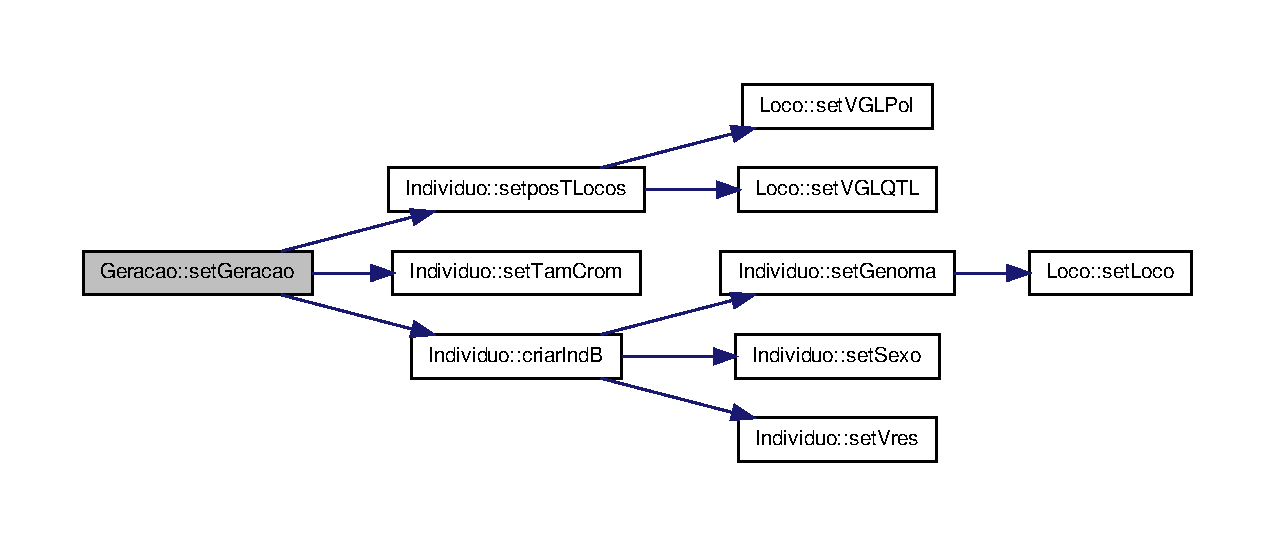
\includegraphics[width=350pt]{class_geracao_ad06d071bed257d62506aa47a5186496f_cgraph}
\end{center}
\end{figure}




\-Este é o diagrama das funções que utilizam esta função\-:\nopagebreak
\begin{figure}[H]
\begin{center}
\leavevmode
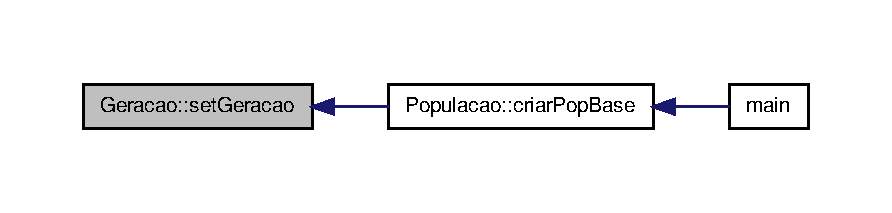
\includegraphics[width=350pt]{class_geracao_ad06d071bed257d62506aa47a5186496f_icgraph}
\end{center}
\end{figure}


\hypertarget{class_geracao_adc9964b180ec37ecf40ba517a88f2c55}{\index{\-Geracao@{\-Geracao}!set\-Mediag@{set\-Mediag}}
\index{set\-Mediag@{set\-Mediag}!Geracao@{\-Geracao}}
\subsubsection[{set\-Mediag}]{\setlength{\rightskip}{0pt plus 5cm}void {\bf \-Geracao\-::set\-Mediag} (
\begin{DoxyParamCaption}
{}
\end{DoxyParamCaption}
)}}\label{class_geracao_adc9964b180ec37ecf40ba517a88f2c55}
\-Ajusta a media da caracteristica na geracao. \hypertarget{class_geracao_affc43315799b830a85c176072c5607ae}{\index{\-Geracao@{\-Geracao}!set\-Varadg@{set\-Varadg}}
\index{set\-Varadg@{set\-Varadg}!Geracao@{\-Geracao}}
\subsubsection[{set\-Varadg}]{\setlength{\rightskip}{0pt plus 5cm}void {\bf \-Geracao\-::set\-Varadg} (
\begin{DoxyParamCaption}
{}
\end{DoxyParamCaption}
)}}\label{class_geracao_affc43315799b830a85c176072c5607ae}
\-Ajusta a variancia genetica aditiva da caracterista na geracao. \hypertarget{class_geracao_a8b139af5fcd3e5c5b302720cd6cabea0}{\index{\-Geracao@{\-Geracao}!set\-Varresg@{set\-Varresg}}
\index{set\-Varresg@{set\-Varresg}!Geracao@{\-Geracao}}
\subsubsection[{set\-Varresg}]{\setlength{\rightskip}{0pt plus 5cm}void {\bf \-Geracao\-::set\-Varresg} (
\begin{DoxyParamCaption}
{}
\end{DoxyParamCaption}
)}}\label{class_geracao_a8b139af5fcd3e5c5b302720cd6cabea0}
\-Ajusta a variancia residual (ambiente) da caracteristica na geracao. 

\-A documentação para esta classe foi gerada a partir dos seguintes ficheiros\-:\begin{DoxyCompactItemize}
\item 
/home/michel/workspace/\-L\-Z5/\hyperlink{geracao_8h}{geracao.\-h}\item 
/home/michel/workspace/\-L\-Z5/\hyperlink{geracao_8cpp}{geracao.\-cpp}\end{DoxyCompactItemize}

\hypertarget{class_individuo}{\section{\-Referência à classe \-Individuo}
\label{class_individuo}\index{\-Individuo@{\-Individuo}}
}


\-Cria um genoma que constitui um individuo.  




{\ttfamily \#include $<$individuo.\-h$>$}

\subsection*{\-Membros públicos}
\begin{DoxyCompactItemize}
\item 
\hyperlink{class_individuo_a3042a660b9789ee24dd3658248c8e0b9}{\-Individuo} ()
\item 
void \hyperlink{class_individuo_a93f10457d66068fe4e358a495d2e494c}{criar\-Ind\-B} (bool tipoid, float varres, float mediavarres)
\item 
void \hyperlink{class_individuo_ae89912e2bcf4391c30d6a5074f709c88}{setpos\-T\-Locos} (unsigned int qtdlocos, unsigned int qtdqtl, unsigned int qtdmarcador, float varad, float freqp, float freqpqtl, float pvaqtl)
\item 
void \hyperlink{class_individuo_a1641427ff59310a53fc0076e519102c6}{set\-Genoma} (bool tipoid)
\item 
void \hyperlink{class_individuo_a2366e00f66ed23bd142a1d63509098e4}{set\-Tam\-Crom} (unsigned int qtdlocos, unsigned int qtdcrom)
\item 
void \hyperlink{class_individuo_a3271e903e8edcb3bac726a0b3ff1d1a7}{set\-Vres} (float varres, float mediavarres)
\item 
float \hyperlink{class_individuo_a602f0cf13154ca33b265b7d59b494ed3}{get\-Vad} ()
\item 
void \hyperlink{class_individuo_a40f1b7aaf7abc0e1e272eab2e7074fbd}{set\-Sexo} ()
\item 
vector$<$ unsigned int $>$ \hyperlink{class_individuo_a7aae9dafaa8ffebe2c20bd73ef7133cc}{getpos\-T\-Locos} ()
\item 
vector$<$ \hyperlink{class_loco}{\-Loco} $\ast$ $>$ \hyperlink{class_individuo_ac724222b106e77476ee0247ad170383d}{get\-Genoma} ()
\item 
unsigned int \hyperlink{class_individuo_a17aa04fe0128e944416d52d7c1867638}{get\-Id} ()
\item 
unsigned int \hyperlink{class_individuo_a43a77e5804d60b1943799e0299d34357}{get\-Idp} ()
\item 
unsigned int \hyperlink{class_individuo_a60ec384d3937146ab8353d3ebc715f6b}{get\-Idm} ()
\item 
bool \hyperlink{class_individuo_af6b53d0812f8ed281de665877a256498}{get\-Sexo} ()
\item 
float \hyperlink{class_individuo_a205f982134fd0df2f951946743e1c2b6}{get\-Vres} ()
\item 
float \hyperlink{class_individuo_a7a18d46c7f802c31a353db09035e2f2b}{get\-Fen} ()
\end{DoxyCompactItemize}


\subsection{\-Descrição detalhada}
\-Cria um genoma que constitui um individuo. 

\-A classe \hyperlink{class_individuo}{\-Individuo} tem como funcao armazenar o genoma, que ira compor o individuo e armazenar tambem as informacoes de identificacao, como o \-I\-D do individuo e os \-I\-Ds dos pais, bem como o sexo do indivíduo e o valor do efeito residual, referente a um erro aleatorio de ambiente. 

\subsection{\-Documentação dos \-Construtores \& \-Destrutor}
\hypertarget{class_individuo_a3042a660b9789ee24dd3658248c8e0b9}{\index{\-Individuo@{\-Individuo}!\-Individuo@{\-Individuo}}
\index{\-Individuo@{\-Individuo}!Individuo@{\-Individuo}}
\subsubsection[{\-Individuo}]{\setlength{\rightskip}{0pt plus 5cm}{\bf \-Individuo\-::\-Individuo} (
\begin{DoxyParamCaption}
{}
\end{DoxyParamCaption}
)\hspace{0.3cm}{\ttfamily  \mbox{[}inline\mbox{]}}}}\label{class_individuo_a3042a660b9789ee24dd3658248c8e0b9}
\-Cria um objeto do tipo \-Idividuo com sexo (false), o id (cont\-\_\-id), idp (0), idm (0) e vres (0). 

\subsection{\-Documentação dos métodos}
\hypertarget{class_individuo_a93f10457d66068fe4e358a495d2e494c}{\index{\-Individuo@{\-Individuo}!criar\-Ind\-B@{criar\-Ind\-B}}
\index{criar\-Ind\-B@{criar\-Ind\-B}!Individuo@{\-Individuo}}
\subsubsection[{criar\-Ind\-B}]{\setlength{\rightskip}{0pt plus 5cm}void {\bf \-Individuo\-::criar\-Ind\-B} (
\begin{DoxyParamCaption}
\item[{bool}]{tipoid, }
\item[{float}]{varres, }
\item[{float}]{mediavarres}
\end{DoxyParamCaption}
)}}\label{class_individuo_a93f10457d66068fe4e358a495d2e494c}
\-Metodo para criar um individuo da \hyperlink{class_populacao}{\-Populacao} \-Base. 
\begin{DoxyParams}{\-Parâmetros}
{\em tipoid} & -\/ corresponde ao tipo de alelo a ser criado (0 -\/ sem identificacao, 1 -\/ com identificacao); \\
\hline
{\em varres} & -\/ \-Variancia residual fornecida pelo usuario; \\
\hline
{\em mediavarres} & -\/ \-Media da variancia residual fornecida pelo usuario. \\
\hline
\end{DoxyParams}


\-Grafo de chamadas desta função\-:\nopagebreak
\begin{figure}[H]
\begin{center}
\leavevmode
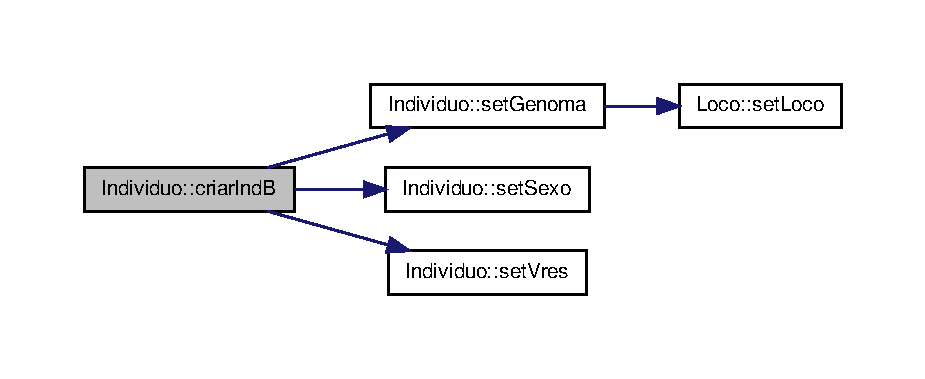
\includegraphics[width=350pt]{class_individuo_a93f10457d66068fe4e358a495d2e494c_cgraph}
\end{center}
\end{figure}




\-Este é o diagrama das funções que utilizam esta função\-:\nopagebreak
\begin{figure}[H]
\begin{center}
\leavevmode
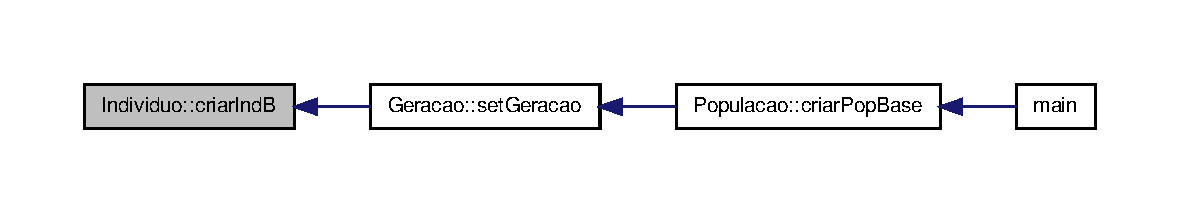
\includegraphics[width=350pt]{class_individuo_a93f10457d66068fe4e358a495d2e494c_icgraph}
\end{center}
\end{figure}


\hypertarget{class_individuo_a7a18d46c7f802c31a353db09035e2f2b}{\index{\-Individuo@{\-Individuo}!get\-Fen@{get\-Fen}}
\index{get\-Fen@{get\-Fen}!Individuo@{\-Individuo}}
\subsubsection[{get\-Fen}]{\setlength{\rightskip}{0pt plus 5cm}float {\bf \-Individuo\-::get\-Fen} (
\begin{DoxyParamCaption}
{}
\end{DoxyParamCaption}
)\hspace{0.3cm}{\ttfamily  \mbox{[}inline\mbox{]}}}}\label{class_individuo_a7a18d46c7f802c31a353db09035e2f2b}


\-Grafo de chamadas desta função\-:\nopagebreak
\begin{figure}[H]
\begin{center}
\leavevmode
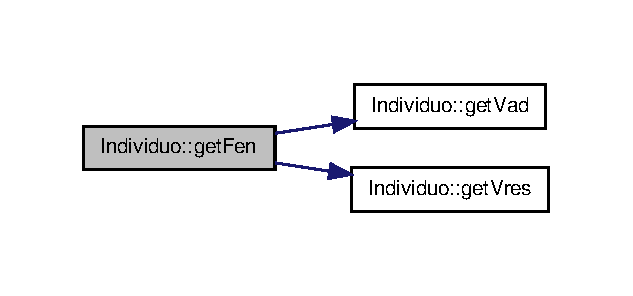
\includegraphics[width=304pt]{class_individuo_a7a18d46c7f802c31a353db09035e2f2b_cgraph}
\end{center}
\end{figure}


\hypertarget{class_individuo_ac724222b106e77476ee0247ad170383d}{\index{\-Individuo@{\-Individuo}!get\-Genoma@{get\-Genoma}}
\index{get\-Genoma@{get\-Genoma}!Individuo@{\-Individuo}}
\subsubsection[{get\-Genoma}]{\setlength{\rightskip}{0pt plus 5cm}vector$<${\bf \-Loco}$\ast$$>$ {\bf \-Individuo\-::get\-Genoma} (
\begin{DoxyParamCaption}
{}
\end{DoxyParamCaption}
)\hspace{0.3cm}{\ttfamily  \mbox{[}inline\mbox{]}}}}\label{class_individuo_ac724222b106e77476ee0247ad170383d}
\-Retorna o genoma do individuo. \hypertarget{class_individuo_a17aa04fe0128e944416d52d7c1867638}{\index{\-Individuo@{\-Individuo}!get\-Id@{get\-Id}}
\index{get\-Id@{get\-Id}!Individuo@{\-Individuo}}
\subsubsection[{get\-Id}]{\setlength{\rightskip}{0pt plus 5cm}unsigned int {\bf \-Individuo\-::get\-Id} (
\begin{DoxyParamCaption}
{}
\end{DoxyParamCaption}
)\hspace{0.3cm}{\ttfamily  \mbox{[}inline\mbox{]}}}}\label{class_individuo_a17aa04fe0128e944416d52d7c1867638}
\-Retorna o \-I\-D do individuo. \hypertarget{class_individuo_a60ec384d3937146ab8353d3ebc715f6b}{\index{\-Individuo@{\-Individuo}!get\-Idm@{get\-Idm}}
\index{get\-Idm@{get\-Idm}!Individuo@{\-Individuo}}
\subsubsection[{get\-Idm}]{\setlength{\rightskip}{0pt plus 5cm}unsigned int {\bf \-Individuo\-::get\-Idm} (
\begin{DoxyParamCaption}
{}
\end{DoxyParamCaption}
)\hspace{0.3cm}{\ttfamily  \mbox{[}inline\mbox{]}}}}\label{class_individuo_a60ec384d3937146ab8353d3ebc715f6b}
\-Retorna o \-I\-D da mae do individuo. \hypertarget{class_individuo_a43a77e5804d60b1943799e0299d34357}{\index{\-Individuo@{\-Individuo}!get\-Idp@{get\-Idp}}
\index{get\-Idp@{get\-Idp}!Individuo@{\-Individuo}}
\subsubsection[{get\-Idp}]{\setlength{\rightskip}{0pt plus 5cm}unsigned int {\bf \-Individuo\-::get\-Idp} (
\begin{DoxyParamCaption}
{}
\end{DoxyParamCaption}
)\hspace{0.3cm}{\ttfamily  \mbox{[}inline\mbox{]}}}}\label{class_individuo_a43a77e5804d60b1943799e0299d34357}
\-Retorna o \-I\-D do pai do individuo. \hypertarget{class_individuo_a7aae9dafaa8ffebe2c20bd73ef7133cc}{\index{\-Individuo@{\-Individuo}!getpos\-T\-Locos@{getpos\-T\-Locos}}
\index{getpos\-T\-Locos@{getpos\-T\-Locos}!Individuo@{\-Individuo}}
\subsubsection[{getpos\-T\-Locos}]{\setlength{\rightskip}{0pt plus 5cm}vector$<$unsigned int$>$ {\bf \-Individuo\-::getpos\-T\-Locos} (
\begin{DoxyParamCaption}
{}
\end{DoxyParamCaption}
)\hspace{0.3cm}{\ttfamily  \mbox{[}inline\mbox{]}}}}\label{class_individuo_a7aae9dafaa8ffebe2c20bd73ef7133cc}
\-Retorna o vetor de configuracao do genoma da populacao. \hypertarget{class_individuo_af6b53d0812f8ed281de665877a256498}{\index{\-Individuo@{\-Individuo}!get\-Sexo@{get\-Sexo}}
\index{get\-Sexo@{get\-Sexo}!Individuo@{\-Individuo}}
\subsubsection[{get\-Sexo}]{\setlength{\rightskip}{0pt plus 5cm}bool {\bf \-Individuo\-::get\-Sexo} (
\begin{DoxyParamCaption}
{}
\end{DoxyParamCaption}
)\hspace{0.3cm}{\ttfamily  \mbox{[}inline\mbox{]}}}}\label{class_individuo_af6b53d0812f8ed281de665877a256498}
\-Retorna o sexo do individuo. \hypertarget{class_individuo_a602f0cf13154ca33b265b7d59b494ed3}{\index{\-Individuo@{\-Individuo}!get\-Vad@{get\-Vad}}
\index{get\-Vad@{get\-Vad}!Individuo@{\-Individuo}}
\subsubsection[{get\-Vad}]{\setlength{\rightskip}{0pt plus 5cm}float {\bf \-Individuo\-::get\-Vad} (
\begin{DoxyParamCaption}
{}
\end{DoxyParamCaption}
)}}\label{class_individuo_a602f0cf13154ca33b265b7d59b494ed3}
\-Retorna um float com o \-Valor \-Genetico \-Aditivo do individuo. 

\-Este é o diagrama das funções que utilizam esta função\-:\nopagebreak
\begin{figure}[H]
\begin{center}
\leavevmode
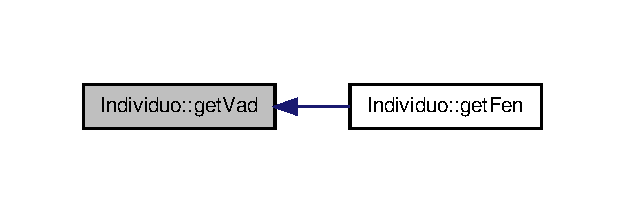
\includegraphics[width=300pt]{class_individuo_a602f0cf13154ca33b265b7d59b494ed3_icgraph}
\end{center}
\end{figure}


\hypertarget{class_individuo_a205f982134fd0df2f951946743e1c2b6}{\index{\-Individuo@{\-Individuo}!get\-Vres@{get\-Vres}}
\index{get\-Vres@{get\-Vres}!Individuo@{\-Individuo}}
\subsubsection[{get\-Vres}]{\setlength{\rightskip}{0pt plus 5cm}float {\bf \-Individuo\-::get\-Vres} (
\begin{DoxyParamCaption}
{}
\end{DoxyParamCaption}
)\hspace{0.3cm}{\ttfamily  \mbox{[}inline\mbox{]}}}}\label{class_individuo_a205f982134fd0df2f951946743e1c2b6}
\-Retorna o \-Valor de efeito de ambiente (residual) do individuo. 

\-Este é o diagrama das funções que utilizam esta função\-:\nopagebreak
\begin{figure}[H]
\begin{center}
\leavevmode
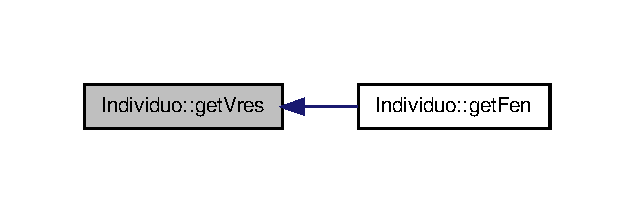
\includegraphics[width=304pt]{class_individuo_a205f982134fd0df2f951946743e1c2b6_icgraph}
\end{center}
\end{figure}


\hypertarget{class_individuo_a1641427ff59310a53fc0076e519102c6}{\index{\-Individuo@{\-Individuo}!set\-Genoma@{set\-Genoma}}
\index{set\-Genoma@{set\-Genoma}!Individuo@{\-Individuo}}
\subsubsection[{set\-Genoma}]{\setlength{\rightskip}{0pt plus 5cm}void {\bf \-Individuo\-::set\-Genoma} (
\begin{DoxyParamCaption}
\item[{bool}]{tipoid}
\end{DoxyParamCaption}
)}}\label{class_individuo_a1641427ff59310a53fc0076e519102c6}
\-Metodo para criar o genoma do individuo. 
\begin{DoxyParams}{\-Parâmetros}
{\em tipoid} & -\/ \-Ver \hyperlink{class_loco_a17e42d11b5d0f86797f942742c476f04}{\-Loco\-::set\-Loco()} da classe \hyperlink{class_loco}{\-Loco}. \\
\hline
\end{DoxyParams}


\-Grafo de chamadas desta função\-:\nopagebreak
\begin{figure}[H]
\begin{center}
\leavevmode
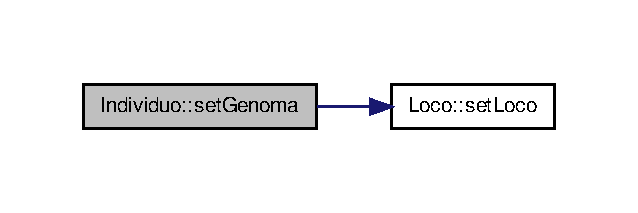
\includegraphics[width=306pt]{class_individuo_a1641427ff59310a53fc0076e519102c6_cgraph}
\end{center}
\end{figure}




\-Este é o diagrama das funções que utilizam esta função\-:\nopagebreak
\begin{figure}[H]
\begin{center}
\leavevmode
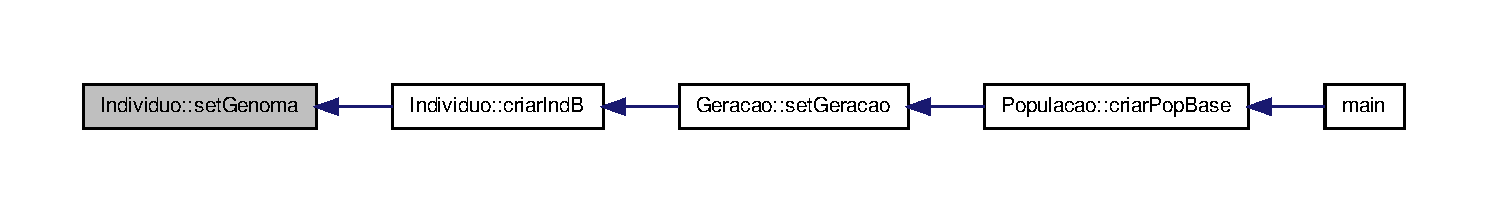
\includegraphics[width=350pt]{class_individuo_a1641427ff59310a53fc0076e519102c6_icgraph}
\end{center}
\end{figure}


\hypertarget{class_individuo_ae89912e2bcf4391c30d6a5074f709c88}{\index{\-Individuo@{\-Individuo}!setpos\-T\-Locos@{setpos\-T\-Locos}}
\index{setpos\-T\-Locos@{setpos\-T\-Locos}!Individuo@{\-Individuo}}
\subsubsection[{setpos\-T\-Locos}]{\setlength{\rightskip}{0pt plus 5cm}void {\bf \-Individuo\-::setpos\-T\-Locos} (
\begin{DoxyParamCaption}
\item[{unsigned int}]{qtdlocos, }
\item[{unsigned int}]{qtdqtl, }
\item[{unsigned int}]{qtdmarcador, }
\item[{float}]{varad, }
\item[{float}]{freqp, }
\item[{float}]{freqpqtl, }
\item[{float}]{pvaqtl}
\end{DoxyParamCaption}
)}}\label{class_individuo_ae89912e2bcf4391c30d6a5074f709c88}
\-Metodo para criar as posicoes do diferentes tipos de locos, um vetor static, apresentando a mesma configuracao para todos os individuos durante todo o processo de simulacao, cria tambem os vetores de efeito de contribuicao para cada loco poligenico e \-Q\-T\-L. \-Esta funcao eh chamada apenas uma vez, no inicio da simulacao. 
\begin{DoxyParams}{\-Parâmetros}
{\em qtdlocos} & -\/ ver \hyperlink{class_loco_a350c5bd93d8ca9d4f312555e27891bf4}{\-Loco\-::set\-V\-G\-L\-Pol()}; \\
\hline
{\em qtdqtl} & -\/ ver \hyperlink{class_loco_a350c5bd93d8ca9d4f312555e27891bf4}{\-Loco\-::set\-V\-G\-L\-Pol()}; \\
\hline
{\em qtdmarcador} & -\/ ver \hyperlink{class_loco_a350c5bd93d8ca9d4f312555e27891bf4}{\-Loco\-::set\-V\-G\-L\-Pol()}; \\
\hline
{\em varad} & -\/ ver \hyperlink{class_loco_a350c5bd93d8ca9d4f312555e27891bf4}{\-Loco\-::set\-V\-G\-L\-Pol()}; \\
\hline
{\em freqp} & -\/ ver \hyperlink{class_loco_a350c5bd93d8ca9d4f312555e27891bf4}{\-Loco\-::set\-V\-G\-L\-Pol()}; \\
\hline
{\em freqpqtl} & -\/ ver \hyperlink{class_loco_a0a3371328be88138be0386897264931e}{\-Loco\-::set\-V\-G\-L\-Q\-T\-L()}; \\
\hline
{\em pvaqtl} & -\/ ver \hyperlink{class_loco_a350c5bd93d8ca9d4f312555e27891bf4}{\-Loco\-::set\-V\-G\-L\-Pol()}; \\
\hline
\end{DoxyParams}


\-Grafo de chamadas desta função\-:\nopagebreak
\begin{figure}[H]
\begin{center}
\leavevmode
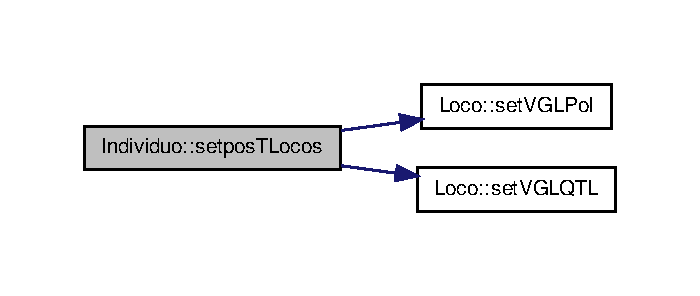
\includegraphics[width=336pt]{class_individuo_ae89912e2bcf4391c30d6a5074f709c88_cgraph}
\end{center}
\end{figure}




\-Este é o diagrama das funções que utilizam esta função\-:\nopagebreak
\begin{figure}[H]
\begin{center}
\leavevmode
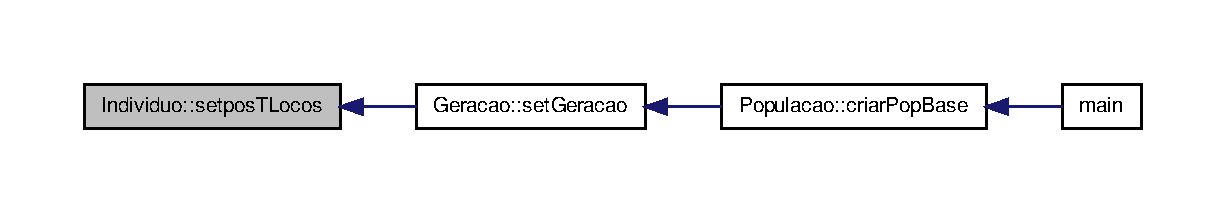
\includegraphics[width=350pt]{class_individuo_ae89912e2bcf4391c30d6a5074f709c88_icgraph}
\end{center}
\end{figure}


\hypertarget{class_individuo_a40f1b7aaf7abc0e1e272eab2e7074fbd}{\index{\-Individuo@{\-Individuo}!set\-Sexo@{set\-Sexo}}
\index{set\-Sexo@{set\-Sexo}!Individuo@{\-Individuo}}
\subsubsection[{set\-Sexo}]{\setlength{\rightskip}{0pt plus 5cm}void {\bf \-Individuo\-::set\-Sexo} (
\begin{DoxyParamCaption}
{}
\end{DoxyParamCaption}
)\hspace{0.3cm}{\ttfamily  \mbox{[}inline\mbox{]}}}}\label{class_individuo_a40f1b7aaf7abc0e1e272eab2e7074fbd}
\-Altera o valor do sexo para \-T\-R\-U\-E. 

\-Este é o diagrama das funções que utilizam esta função\-:\nopagebreak
\begin{figure}[H]
\begin{center}
\leavevmode
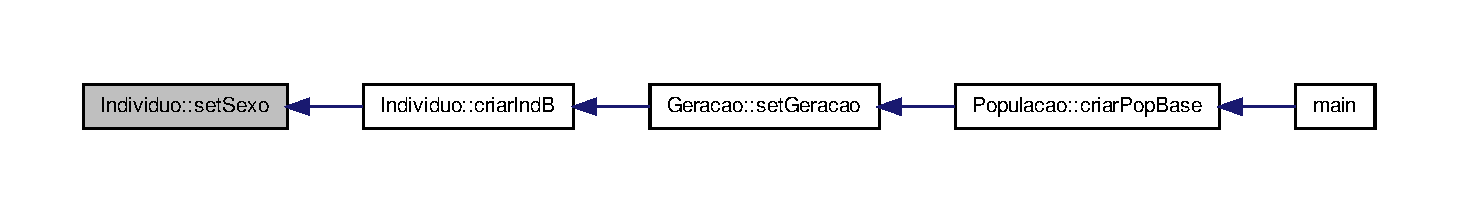
\includegraphics[width=350pt]{class_individuo_a40f1b7aaf7abc0e1e272eab2e7074fbd_icgraph}
\end{center}
\end{figure}


\hypertarget{class_individuo_a2366e00f66ed23bd142a1d63509098e4}{\index{\-Individuo@{\-Individuo}!set\-Tam\-Crom@{set\-Tam\-Crom}}
\index{set\-Tam\-Crom@{set\-Tam\-Crom}!Individuo@{\-Individuo}}
\subsubsection[{set\-Tam\-Crom}]{\setlength{\rightskip}{0pt plus 5cm}void {\bf \-Individuo\-::set\-Tam\-Crom} (
\begin{DoxyParamCaption}
\item[{unsigned int}]{qtdlocos, }
\item[{unsigned int}]{qtdcrom}
\end{DoxyParamCaption}
)}}\label{class_individuo_a2366e00f66ed23bd142a1d63509098e4}
\-Metodo para criar vetor static com o tamanho dos cromossomos. (\-O simulador esta ajustando todos os cromossomos com o mesmo tamanho!) 
\begin{DoxyParams}{\-Parâmetros}
{\em qtdlocos} & -\/ \-Quantidade total de locos que ira compor o genoma do individuo; \\
\hline
{\em qtdcrom} & -\/ \-Quantidade de cromossomos que ira compor o individuo; \\
\hline
\end{DoxyParams}


\-Este é o diagrama das funções que utilizam esta função\-:\nopagebreak
\begin{figure}[H]
\begin{center}
\leavevmode
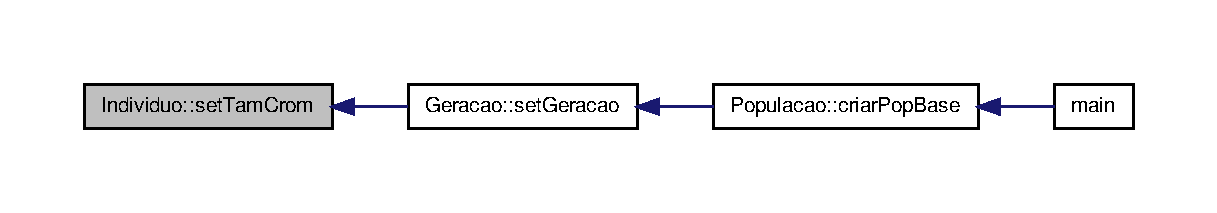
\includegraphics[width=350pt]{class_individuo_a2366e00f66ed23bd142a1d63509098e4_icgraph}
\end{center}
\end{figure}


\hypertarget{class_individuo_a3271e903e8edcb3bac726a0b3ff1d1a7}{\index{\-Individuo@{\-Individuo}!set\-Vres@{set\-Vres}}
\index{set\-Vres@{set\-Vres}!Individuo@{\-Individuo}}
\subsubsection[{set\-Vres}]{\setlength{\rightskip}{0pt plus 5cm}void {\bf \-Individuo\-::set\-Vres} (
\begin{DoxyParamCaption}
\item[{float}]{varres, }
\item[{float}]{mediavarres}
\end{DoxyParamCaption}
)}}\label{class_individuo_a3271e903e8edcb3bac726a0b3ff1d1a7}
\-Ajusta o \-Valor de efeito residual (nao genetico) do individuo. 
\begin{DoxyParams}{\-Parâmetros}
{\em varres} & -\/ \-Variancia residual da populacao; \\
\hline
{\em mediavarres} & -\/ \-Media da variancia residual da populacao. \\
\hline
\end{DoxyParams}


\-Este é o diagrama das funções que utilizam esta função\-:\nopagebreak
\begin{figure}[H]
\begin{center}
\leavevmode
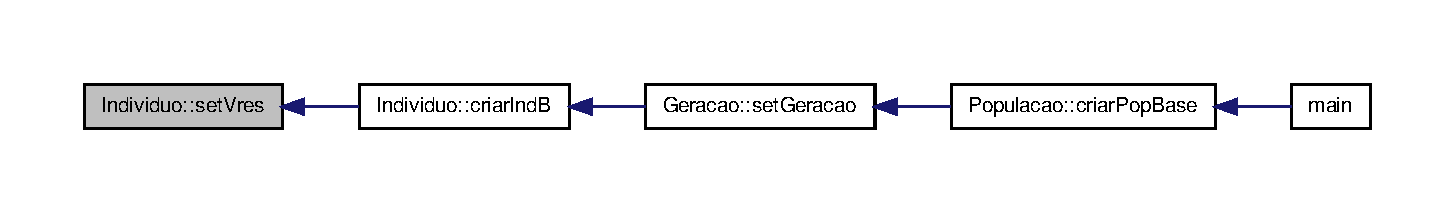
\includegraphics[width=350pt]{class_individuo_a3271e903e8edcb3bac726a0b3ff1d1a7_icgraph}
\end{center}
\end{figure}




\-A documentação para esta classe foi gerada a partir dos seguintes ficheiros\-:\begin{DoxyCompactItemize}
\item 
/home/michel/workspace/\-L\-Z5/\hyperlink{individuo_8h}{individuo.\-h}\item 
/home/michel/workspace/\-L\-Z5/\hyperlink{individuo_8cpp}{individuo.\-cpp}\end{DoxyCompactItemize}

\hypertarget{class_loco}{\section{\-Referência à classe \-Loco}
\label{class_loco}\index{\-Loco@{\-Loco}}
}


\-Classe para criar um \hyperlink{class_loco}{\-Loco} a partir de 2 \-Alelos.  




{\ttfamily \#include $<$loco.\-h$>$}

\subsection*{\-Membros públicos}
\begin{DoxyCompactItemize}
\item 
\hyperlink{class_loco_ac76b405e7b9a8b427f13c92e21dbb749}{\-Loco} ()
\item 
vector$<$ \hyperlink{class_alelo}{\-Alelo} $\ast$ $>$ \hyperlink{class_loco_a710976ac6340a8a4eae1509ddb622f99}{get\-Loco} ()
\item 
float \hyperlink{class_loco_a2f83ae2640e39e14a994d244f3878029}{get\-V\-G\-Lpol} (unsigned int i)
\item 
float \hyperlink{class_loco_a110a570e49a0007ffc6dc5a4269a11aa}{get\-V\-G\-L\-Q\-T\-L} (unsigned int i)
\item 
void \hyperlink{class_loco_a17e42d11b5d0f86797f942742c476f04}{set\-Loco} (bool tipo)
\item 
void \hyperlink{class_loco_a350c5bd93d8ca9d4f312555e27891bf4}{set\-V\-G\-L\-Pol} (float varad, unsigned int qtdlocos, unsigned int qtdqtl, unsigned int qtdmarcador, float freqp, float pvaqtl)
\item 
void \hyperlink{class_loco_a0a3371328be88138be0386897264931e}{set\-V\-G\-L\-Q\-T\-L} (float varad, unsigned int qtdlqtl, float freqpqtl, float pvaqtl)
\end{DoxyCompactItemize}


\subsection{\-Descrição detalhada}
\-Classe para criar um \hyperlink{class_loco}{\-Loco} a partir de 2 \-Alelos. 

\-A \-Classe \hyperlink{class_loco}{\-Loco} tem como funcao armazenar o genotipo (configuracao alelica) de cada loco que ira compor um individuo, nao importando o tipo de loco (marcador, \-Q\-T\-L ou poligenico). \begin{DoxyAuthor}{\-Autor}
\-Michel \-Marques \-Farah e \-Ricardo da \-Fonseca 
\end{DoxyAuthor}
\begin{DoxySince}{\-Desde}
20/09/2012 
\end{DoxySince}
\begin{DoxyVersion}{\-Versão}
1.\-1 
\end{DoxyVersion}


\subsection{\-Documentação dos \-Construtores \& \-Destrutor}
\hypertarget{class_loco_ac76b405e7b9a8b427f13c92e21dbb749}{\index{\-Loco@{\-Loco}!\-Loco@{\-Loco}}
\index{\-Loco@{\-Loco}!Loco@{\-Loco}}
\subsubsection[{\-Loco}]{\setlength{\rightskip}{0pt plus 5cm}{\bf \-Loco\-::\-Loco} (
\begin{DoxyParamCaption}
{}
\end{DoxyParamCaption}
)\hspace{0.3cm}{\ttfamily  \mbox{[}inline\mbox{]}}}}\label{class_loco_ac76b405e7b9a8b427f13c92e21dbb749}
\-Cria um objeto \-Genotipo vazio. 

\subsection{\-Documentação dos métodos}
\hypertarget{class_loco_a710976ac6340a8a4eae1509ddb622f99}{\index{\-Loco@{\-Loco}!get\-Loco@{get\-Loco}}
\index{get\-Loco@{get\-Loco}!Loco@{\-Loco}}
\subsubsection[{get\-Loco}]{\setlength{\rightskip}{0pt plus 5cm}vector$<${\bf \-Alelo}$\ast$$>$ {\bf \-Loco\-::get\-Loco} (
\begin{DoxyParamCaption}
{}
\end{DoxyParamCaption}
)\hspace{0.3cm}{\ttfamily  \mbox{[}inline\mbox{]}}}}\label{class_loco_a710976ac6340a8a4eae1509ddb622f99}
\-Retorna um vetor com 2 poteiros para dois objetos \hyperlink{class_alelo}{\-Alelo} \hypertarget{class_loco_a2f83ae2640e39e14a994d244f3878029}{\index{\-Loco@{\-Loco}!get\-V\-G\-Lpol@{get\-V\-G\-Lpol}}
\index{get\-V\-G\-Lpol@{get\-V\-G\-Lpol}!Loco@{\-Loco}}
\subsubsection[{get\-V\-G\-Lpol}]{\setlength{\rightskip}{0pt plus 5cm}float {\bf \-Loco\-::get\-V\-G\-Lpol} (
\begin{DoxyParamCaption}
\item[{unsigned int}]{i}
\end{DoxyParamCaption}
)\hspace{0.3cm}{\ttfamily  \mbox{[}inline\mbox{]}}}}\label{class_loco_a2f83ae2640e39e14a994d244f3878029}
\-Metodo para retornar a contribuicao dos locos poligenicos dependendo da sua configuracao alelica 
\begin{DoxyParams}{\-Parâmetros}
{\em i} & -\/ indice que indica a posição no array de contribuicao dos locos poligenicos \\
\hline
\end{DoxyParams}
\hypertarget{class_loco_a110a570e49a0007ffc6dc5a4269a11aa}{\index{\-Loco@{\-Loco}!get\-V\-G\-L\-Q\-T\-L@{get\-V\-G\-L\-Q\-T\-L}}
\index{get\-V\-G\-L\-Q\-T\-L@{get\-V\-G\-L\-Q\-T\-L}!Loco@{\-Loco}}
\subsubsection[{get\-V\-G\-L\-Q\-T\-L}]{\setlength{\rightskip}{0pt plus 5cm}float {\bf \-Loco\-::get\-V\-G\-L\-Q\-T\-L} (
\begin{DoxyParamCaption}
\item[{unsigned int}]{i}
\end{DoxyParamCaption}
)\hspace{0.3cm}{\ttfamily  \mbox{[}inline\mbox{]}}}}\label{class_loco_a110a570e49a0007ffc6dc5a4269a11aa}
\-Metodo para retornar a contribuicao dos locos \-Q\-T\-Ls dependendo da sua configuracao alelica 
\begin{DoxyParams}{\-Parâmetros}
{\em i} & -\/ indice que indica a posição no array de contribuicao dos locos \-Q\-T\-Ls \\
\hline
\end{DoxyParams}
\hypertarget{class_loco_a17e42d11b5d0f86797f942742c476f04}{\index{\-Loco@{\-Loco}!set\-Loco@{set\-Loco}}
\index{set\-Loco@{set\-Loco}!Loco@{\-Loco}}
\subsubsection[{set\-Loco}]{\setlength{\rightskip}{0pt plus 5cm}void {\bf \-Loco\-::set\-Loco} (
\begin{DoxyParamCaption}
\item[{bool}]{tipo}
\end{DoxyParamCaption}
)}}\label{class_loco_a17e42d11b5d0f86797f942742c476f04}
\-Metodo para ajustar a configuracao do loco 
\begin{DoxyParams}{\-Parâmetros}
{\em tipo} & -\/ bool para indicar se ira criar um objeto do tipo \hyperlink{class_alelo}{\-Alelo} (\-F\-A\-L\-S\-E) ou do tipo \hyperlink{class_alelo_id}{\-Alelo\-Id} (\-T\-R\-U\-E) \\
\hline
\end{DoxyParams}


\-Este é o diagrama das funções que utilizam esta função\-:\nopagebreak
\begin{figure}[H]
\begin{center}
\leavevmode
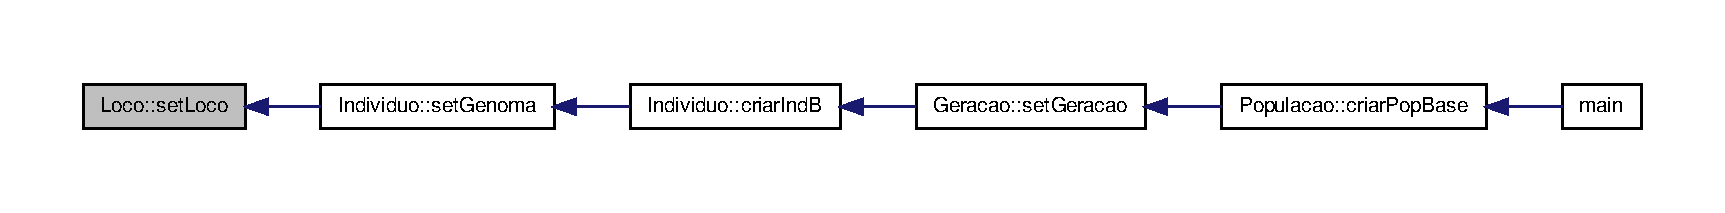
\includegraphics[width=350pt]{class_loco_a17e42d11b5d0f86797f942742c476f04_icgraph}
\end{center}
\end{figure}


\hypertarget{class_loco_a350c5bd93d8ca9d4f312555e27891bf4}{\index{\-Loco@{\-Loco}!set\-V\-G\-L\-Pol@{set\-V\-G\-L\-Pol}}
\index{set\-V\-G\-L\-Pol@{set\-V\-G\-L\-Pol}!Loco@{\-Loco}}
\subsubsection[{set\-V\-G\-L\-Pol}]{\setlength{\rightskip}{0pt plus 5cm}void {\bf \-Loco\-::set\-V\-G\-L\-Pol} (
\begin{DoxyParamCaption}
\item[{float}]{varad, }
\item[{unsigned int}]{qtdlocos, }
\item[{unsigned int}]{qtdqtl, }
\item[{unsigned int}]{qtdmarcador, }
\item[{float}]{freqp, }
\item[{float}]{pvaqtl}
\end{DoxyParamCaption}
)}}\label{class_loco_a350c5bd93d8ca9d4f312555e27891bf4}
\-Metodo para ajustar o vetor static de contribuicao dos locos poligenicos. 
\begin{DoxyParams}{\-Parâmetros}
{\em varad} & -\/ \-Variancia \-Aditiva fornecida pelo usuario; \\
\hline
{\em qtdlocos} & -\/ \-Quantidade de \-Locos \-Poligenicos que irao formar o genoma do individuo; \\
\hline
{\em qtdqtl} & -\/ \-Quantidade de \-Locos \-Q\-T\-Ls que irao formar o genoma do individuo; \\
\hline
{\em qtdmarcador} & -\/ \-Quantidade de \-Locos \-Marcadores no genoma de cada individuo; \\
\hline
{\em freqp} & -\/ \-Frequencia alelica (p) dos locos poligenicos (atribui-\/se a mesma frequencia para todos os locos poligenicos); \\
\hline
{\em pvaqtl} & -\/ \-Proporcao da variancia aditiva que eh explicada pelos \-Q\-T\-Ls. \\
\hline
\end{DoxyParams}


\-Este é o diagrama das funções que utilizam esta função\-:\nopagebreak
\begin{figure}[H]
\begin{center}
\leavevmode
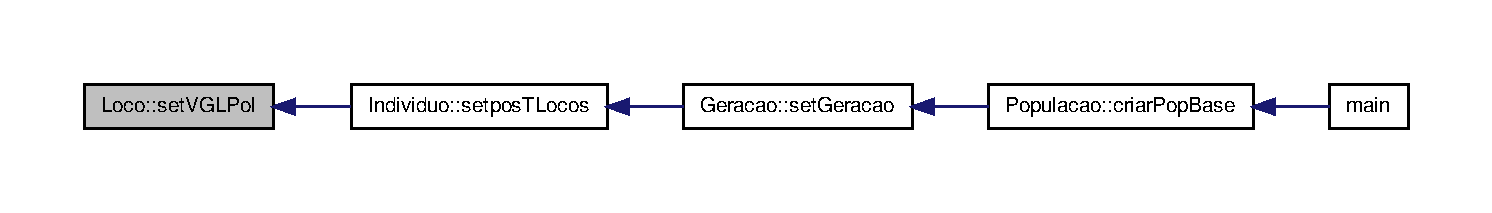
\includegraphics[width=350pt]{class_loco_a350c5bd93d8ca9d4f312555e27891bf4_icgraph}
\end{center}
\end{figure}


\hypertarget{class_loco_a0a3371328be88138be0386897264931e}{\index{\-Loco@{\-Loco}!set\-V\-G\-L\-Q\-T\-L@{set\-V\-G\-L\-Q\-T\-L}}
\index{set\-V\-G\-L\-Q\-T\-L@{set\-V\-G\-L\-Q\-T\-L}!Loco@{\-Loco}}
\subsubsection[{set\-V\-G\-L\-Q\-T\-L}]{\setlength{\rightskip}{0pt plus 5cm}void {\bf \-Loco\-::set\-V\-G\-L\-Q\-T\-L} (
\begin{DoxyParamCaption}
\item[{float}]{varad, }
\item[{unsigned int}]{qtdlqtl, }
\item[{float}]{freqpqtl, }
\item[{float}]{pvaqtl}
\end{DoxyParamCaption}
)}}\label{class_loco_a0a3371328be88138be0386897264931e}
\-Metodo para ajustar o vetor static de contribuicao dos locos \-Q\-T\-Ls. 
\begin{DoxyParams}{\-Parâmetros}
{\em varad} & -\/ \-Variancia \-Aditiva fornecida pelo usuario; \\
\hline
{\em qtdlocos} & -\/ \-Quantidade de \-Locos \-Poligenicos que irao formar o genoma do individuo; \\
\hline
{\em qtdqtl} & -\/ \-Quantidade de \-Locos \-Q\-T\-Ls que irao formar o genoma do individuo; \\
\hline
{\em qtdmarcador} & -\/ \-Quantidade de \-Locos \-Marcadores no genoma de cada individuo; \\
\hline
{\em freqpqtl} & -\/ \-Frequencia alelica (p) dos locos \-Q\-T\-Ls (atribui-\/se a mesma frequencia para todos os locos); \\
\hline
{\em pvaqtl} & -\/ \-Proporcao da variancia aditiva que eh explicada pelos \-Q\-T\-Ls. \\
\hline
\end{DoxyParams}


\-Este é o diagrama das funções que utilizam esta função\-:\nopagebreak
\begin{figure}[H]
\begin{center}
\leavevmode
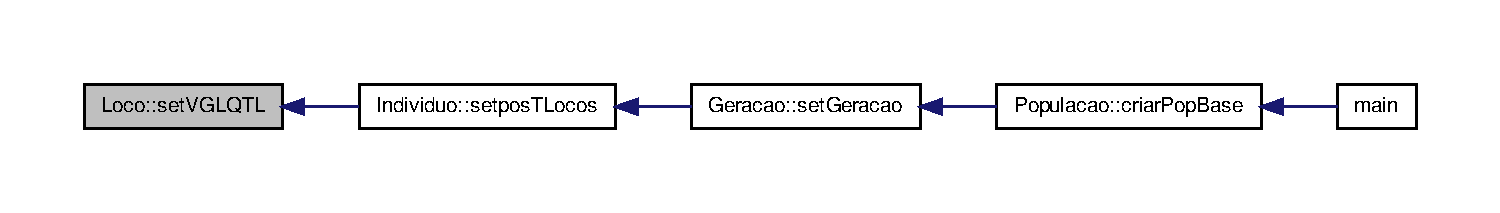
\includegraphics[width=350pt]{class_loco_a0a3371328be88138be0386897264931e_icgraph}
\end{center}
\end{figure}




\-A documentação para esta classe foi gerada a partir dos seguintes ficheiros\-:\begin{DoxyCompactItemize}
\item 
/home/michel/workspace/\-L\-Z5/\hyperlink{loco_8h}{loco.\-h}\item 
/home/michel/workspace/\-L\-Z5/\hyperlink{loco_8cpp}{loco.\-cpp}\end{DoxyCompactItemize}

\hypertarget{class_populacao}{\section{\-Referência à classe \-Populacao}
\label{class_populacao}\index{\-Populacao@{\-Populacao}}
}


\-Cria uma \hyperlink{class_populacao}{\-Populacao}, constituida de diversas \-Geracoes.  




{\ttfamily \#include $<$populacao.\-h$>$}

\subsection*{\-Membros públicos}
\begin{DoxyCompactItemize}
\item 
\hyperlink{class_populacao_ae2b9a4937784998ba732c1453fd1a853}{\-Populacao} ()
\item 
void \hyperlink{class_populacao_a57906fb73eaed4b1eac941d70bd0d9f7}{criar\-Pop\-Base} (unsigned int tampb, bool tipo, float varres, float mediavarres, unsigned int qtdlocos, unsigned int qtdqtl, unsigned int qtdmarcador, float varad, float freqp, float freqpqtl, float pvaqtl, unsigned int qtdcrom)
\item 
float \hyperlink{class_populacao_aa736b42ac4cee186b3f514aec450c168}{get\-Varadp} ()
\item 
float \hyperlink{class_populacao_a48c6fab00206de43f4acae14ae41fd5c}{get\-Varresp} ()
\item 
float \hyperlink{class_populacao_aacb032a00ede3afa9f52a8603abe2ad9}{get\-Varfenp} ()
\item 
void \hyperlink{class_populacao_a1d9fa2673abedcc8b9e69c26fc98f8db}{get\-Mediap} ()
\item 
vector$<$ \hyperlink{class_geracao}{\-Geracao} $\ast$ $>$ \hyperlink{class_populacao_aa7b77ecfe5f2f555887191a324dcd562}{get\-Populacao} ()
\end{DoxyCompactItemize}


\subsection{\-Descrição detalhada}
\-Cria uma \hyperlink{class_populacao}{\-Populacao}, constituida de diversas \-Geracoes. 

\-A classe \hyperlink{class_populacao}{\-Populacao} tem como funcao armazenar as diversas geracoes simuladas, bem como retornar os parametros geneticos e populacionais da populacao simulada. 

\subsection{\-Documentação dos \-Construtores \& \-Destrutor}
\hypertarget{class_populacao_ae2b9a4937784998ba732c1453fd1a853}{\index{\-Populacao@{\-Populacao}!\-Populacao@{\-Populacao}}
\index{\-Populacao@{\-Populacao}!Populacao@{\-Populacao}}
\subsubsection[{\-Populacao}]{\setlength{\rightskip}{0pt plus 5cm}{\bf \-Populacao\-::\-Populacao} (
\begin{DoxyParamCaption}
{}
\end{DoxyParamCaption}
)\hspace{0.3cm}{\ttfamily  \mbox{[}inline\mbox{]}}}}\label{class_populacao_ae2b9a4937784998ba732c1453fd1a853}


\subsection{\-Documentação dos métodos}
\hypertarget{class_populacao_a57906fb73eaed4b1eac941d70bd0d9f7}{\index{\-Populacao@{\-Populacao}!criar\-Pop\-Base@{criar\-Pop\-Base}}
\index{criar\-Pop\-Base@{criar\-Pop\-Base}!Populacao@{\-Populacao}}
\subsubsection[{criar\-Pop\-Base}]{\setlength{\rightskip}{0pt plus 5cm}void {\bf \-Populacao\-::criar\-Pop\-Base} (
\begin{DoxyParamCaption}
\item[{unsigned int}]{tampb, }
\item[{bool}]{tipo, }
\item[{float}]{varres, }
\item[{float}]{mediavarres, }
\item[{unsigned int}]{qtdlocos, }
\item[{unsigned int}]{qtdqtl, }
\item[{unsigned int}]{qtdmarcador, }
\item[{float}]{varad, }
\item[{float}]{freqp, }
\item[{float}]{freqpqtl, }
\item[{float}]{pvaqtl, }
\item[{unsigned int}]{qtdcrom}
\end{DoxyParamCaption}
)}}\label{class_populacao_a57906fb73eaed4b1eac941d70bd0d9f7}
\-Metodo para criar uma populacao base (geracao 0), que ira constituir os individuos fundadores da populacao simulada. 
\begin{DoxyParams}{\-Parâmetros}
{\em tambp} & -\/ \-Tamanho da populacao base; \\
\hline
{\em tipo} & -\/ ver \hyperlink{class_loco_a17e42d11b5d0f86797f942742c476f04}{\-Loco\-::set\-Loco()}; \\
\hline
{\em varres} & -\/ \-Variancia \-Residual fornecida pelo usuario; \\
\hline
{\em mediavarres} & -\/ \-Media da variancia residual fornecida pelo usuario; \\
\hline
{\em qtdlocos} & -\/ \-Quantidade total de locos que ira constituir o genoma do individuo; \\
\hline
{\em qtdqtl} & -\/ \-Quantidade de locos \-Q\-T\-Ls que ira constituir o genoma do individuo; \\
\hline
{\em qtdmarcador} & -\/ \-Quantidade de locos marcadores no genoma do individuo; \\
\hline
{\em varad} & -\/ \-Variancia genetica aditiva da caracteristica a ser simulada; \\
\hline
{\em freqp} & -\/ ver \hyperlink{class_loco_a350c5bd93d8ca9d4f312555e27891bf4}{\-Loco\-::set\-V\-G\-L\-Pol()}; \\
\hline
{\em freqpqtl} & -\/ ver \hyperlink{class_loco_a0a3371328be88138be0386897264931e}{\-Loco\-::set\-V\-G\-L\-Q\-T\-L()}; \\
\hline
{\em pvaqtl} & -\/ ver \hyperlink{class_loco_a350c5bd93d8ca9d4f312555e27891bf4}{\-Loco\-::set\-V\-G\-L\-Pol()}; \\
\hline
{\em qtdcrom} & -\/ \-Quantidade de cromossomos que ira compor o genoma do individuo. \\
\hline
\end{DoxyParams}


\-Grafo de chamadas desta função\-:\nopagebreak
\begin{figure}[H]
\begin{center}
\leavevmode
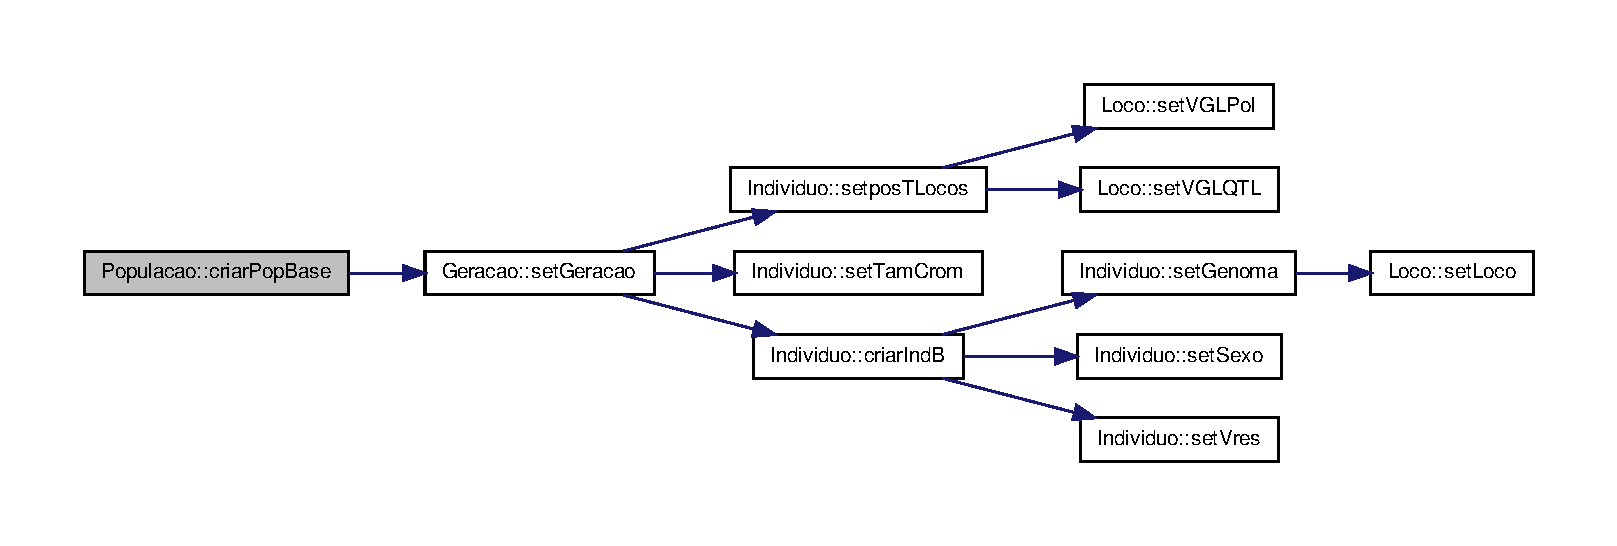
\includegraphics[width=350pt]{class_populacao_a57906fb73eaed4b1eac941d70bd0d9f7_cgraph}
\end{center}
\end{figure}




\-Este é o diagrama das funções que utilizam esta função\-:\nopagebreak
\begin{figure}[H]
\begin{center}
\leavevmode
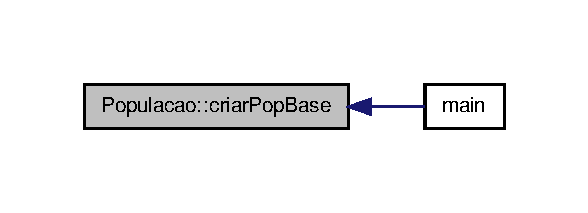
\includegraphics[width=282pt]{class_populacao_a57906fb73eaed4b1eac941d70bd0d9f7_icgraph}
\end{center}
\end{figure}


\hypertarget{class_populacao_a1d9fa2673abedcc8b9e69c26fc98f8db}{\index{\-Populacao@{\-Populacao}!get\-Mediap@{get\-Mediap}}
\index{get\-Mediap@{get\-Mediap}!Populacao@{\-Populacao}}
\subsubsection[{get\-Mediap}]{\setlength{\rightskip}{0pt plus 5cm}void {\bf \-Populacao\-::get\-Mediap} (
\begin{DoxyParamCaption}
{}
\end{DoxyParamCaption}
)}}\label{class_populacao_a1d9fa2673abedcc8b9e69c26fc98f8db}
\-Retorna a media da caracterista na populacao. \hypertarget{class_populacao_aa7b77ecfe5f2f555887191a324dcd562}{\index{\-Populacao@{\-Populacao}!get\-Populacao@{get\-Populacao}}
\index{get\-Populacao@{get\-Populacao}!Populacao@{\-Populacao}}
\subsubsection[{get\-Populacao}]{\setlength{\rightskip}{0pt plus 5cm}vector$<${\bf \-Geracao}$\ast$$>$ {\bf \-Populacao\-::get\-Populacao} (
\begin{DoxyParamCaption}
{}
\end{DoxyParamCaption}
)\hspace{0.3cm}{\ttfamily  \mbox{[}inline\mbox{]}}}}\label{class_populacao_aa7b77ecfe5f2f555887191a324dcd562}
\-Retorna o vetor de geracoes que constitui uma populacao. 

\-Este é o diagrama das funções que utilizam esta função\-:\nopagebreak
\begin{figure}[H]
\begin{center}
\leavevmode
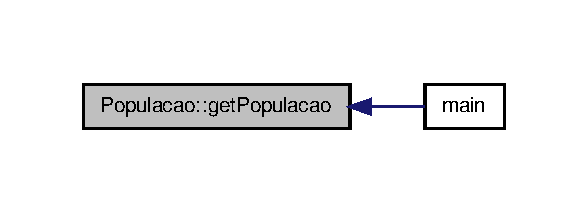
\includegraphics[width=282pt]{class_populacao_aa7b77ecfe5f2f555887191a324dcd562_icgraph}
\end{center}
\end{figure}


\hypertarget{class_populacao_aa736b42ac4cee186b3f514aec450c168}{\index{\-Populacao@{\-Populacao}!get\-Varadp@{get\-Varadp}}
\index{get\-Varadp@{get\-Varadp}!Populacao@{\-Populacao}}
\subsubsection[{get\-Varadp}]{\setlength{\rightskip}{0pt plus 5cm}float {\bf \-Populacao\-::get\-Varadp} (
\begin{DoxyParamCaption}
{}
\end{DoxyParamCaption}
)}}\label{class_populacao_aa736b42ac4cee186b3f514aec450c168}
\-Retorna a variancia genetica aditiva da populacao. 

\-Este é o diagrama das funções que utilizam esta função\-:\nopagebreak
\begin{figure}[H]
\begin{center}
\leavevmode
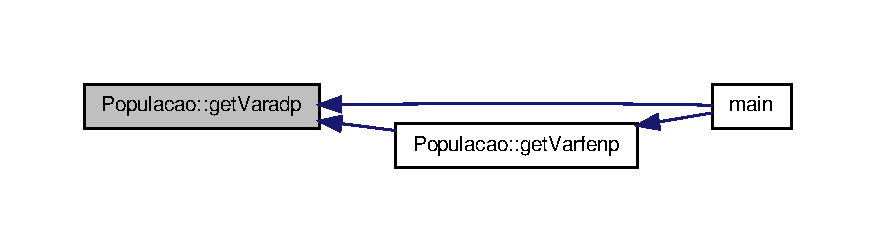
\includegraphics[width=350pt]{class_populacao_aa736b42ac4cee186b3f514aec450c168_icgraph}
\end{center}
\end{figure}


\hypertarget{class_populacao_aacb032a00ede3afa9f52a8603abe2ad9}{\index{\-Populacao@{\-Populacao}!get\-Varfenp@{get\-Varfenp}}
\index{get\-Varfenp@{get\-Varfenp}!Populacao@{\-Populacao}}
\subsubsection[{get\-Varfenp}]{\setlength{\rightskip}{0pt plus 5cm}float {\bf \-Populacao\-::get\-Varfenp} (
\begin{DoxyParamCaption}
{}
\end{DoxyParamCaption}
)}}\label{class_populacao_aacb032a00ede3afa9f52a8603abe2ad9}
\-Retorna a variancia fenotipica da populacao. 

\-Grafo de chamadas desta função\-:\nopagebreak
\begin{figure}[H]
\begin{center}
\leavevmode
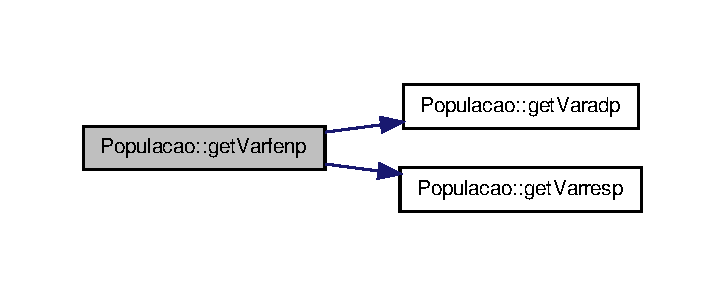
\includegraphics[width=348pt]{class_populacao_aacb032a00ede3afa9f52a8603abe2ad9_cgraph}
\end{center}
\end{figure}




\-Este é o diagrama das funções que utilizam esta função\-:\nopagebreak
\begin{figure}[H]
\begin{center}
\leavevmode
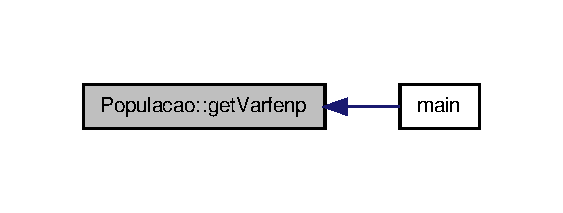
\includegraphics[width=270pt]{class_populacao_aacb032a00ede3afa9f52a8603abe2ad9_icgraph}
\end{center}
\end{figure}


\hypertarget{class_populacao_a48c6fab00206de43f4acae14ae41fd5c}{\index{\-Populacao@{\-Populacao}!get\-Varresp@{get\-Varresp}}
\index{get\-Varresp@{get\-Varresp}!Populacao@{\-Populacao}}
\subsubsection[{get\-Varresp}]{\setlength{\rightskip}{0pt plus 5cm}float {\bf \-Populacao\-::get\-Varresp} (
\begin{DoxyParamCaption}
{}
\end{DoxyParamCaption}
)}}\label{class_populacao_a48c6fab00206de43f4acae14ae41fd5c}
\-Retorna a variancia residual da populacao. 

\-Este é o diagrama das funções que utilizam esta função\-:\nopagebreak
\begin{figure}[H]
\begin{center}
\leavevmode
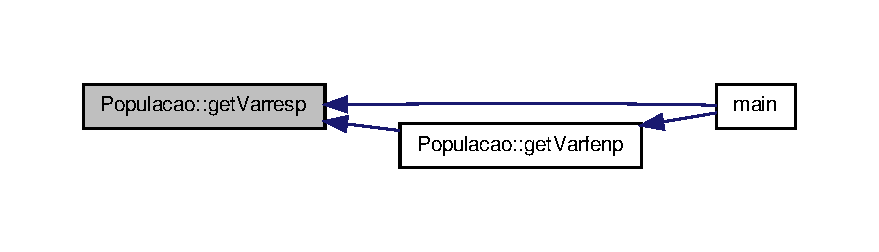
\includegraphics[width=350pt]{class_populacao_a48c6fab00206de43f4acae14ae41fd5c_icgraph}
\end{center}
\end{figure}




\-A documentação para esta classe foi gerada a partir dos seguintes ficheiros\-:\begin{DoxyCompactItemize}
\item 
/home/michel/workspace/\-L\-Z5/\hyperlink{populacao_8h}{populacao.\-h}\item 
/home/michel/workspace/\-L\-Z5/\hyperlink{populacao_8cpp}{populacao.\-cpp}\end{DoxyCompactItemize}

\chapter{\-Documentação do ficheiro}
\hypertarget{alelo_8cpp}{\section{\-Referência ao ficheiro /home/michel/workspace/\-L\-Z5/alelo.cpp}
\label{alelo_8cpp}\index{/home/michel/workspace/\-L\-Z5/alelo.\-cpp@{/home/michel/workspace/\-L\-Z5/alelo.\-cpp}}
}
{\ttfamily \#include \char`\"{}alelo.\-h\char`\"{}}\*
\-Diagrama de dependências de inclusão para alelo.\-cpp\-:\nopagebreak
\begin{figure}[H]
\begin{center}
\leavevmode
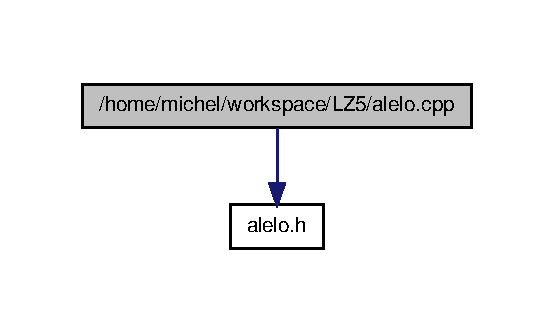
\includegraphics[width=266pt]{alelo_8cpp__incl}
\end{center}
\end{figure}

\hypertarget{alelo_8h}{\section{\-Referência ao ficheiro /home/michel/workspace/\-L\-Z5/alelo.h}
\label{alelo_8h}\index{/home/michel/workspace/\-L\-Z5/alelo.\-h@{/home/michel/workspace/\-L\-Z5/alelo.\-h}}
}
\-Este grafo mostra quais são os ficheiros que incluem directamente ou indirectamente este ficheiro\-:\nopagebreak
\begin{figure}[H]
\begin{center}
\leavevmode
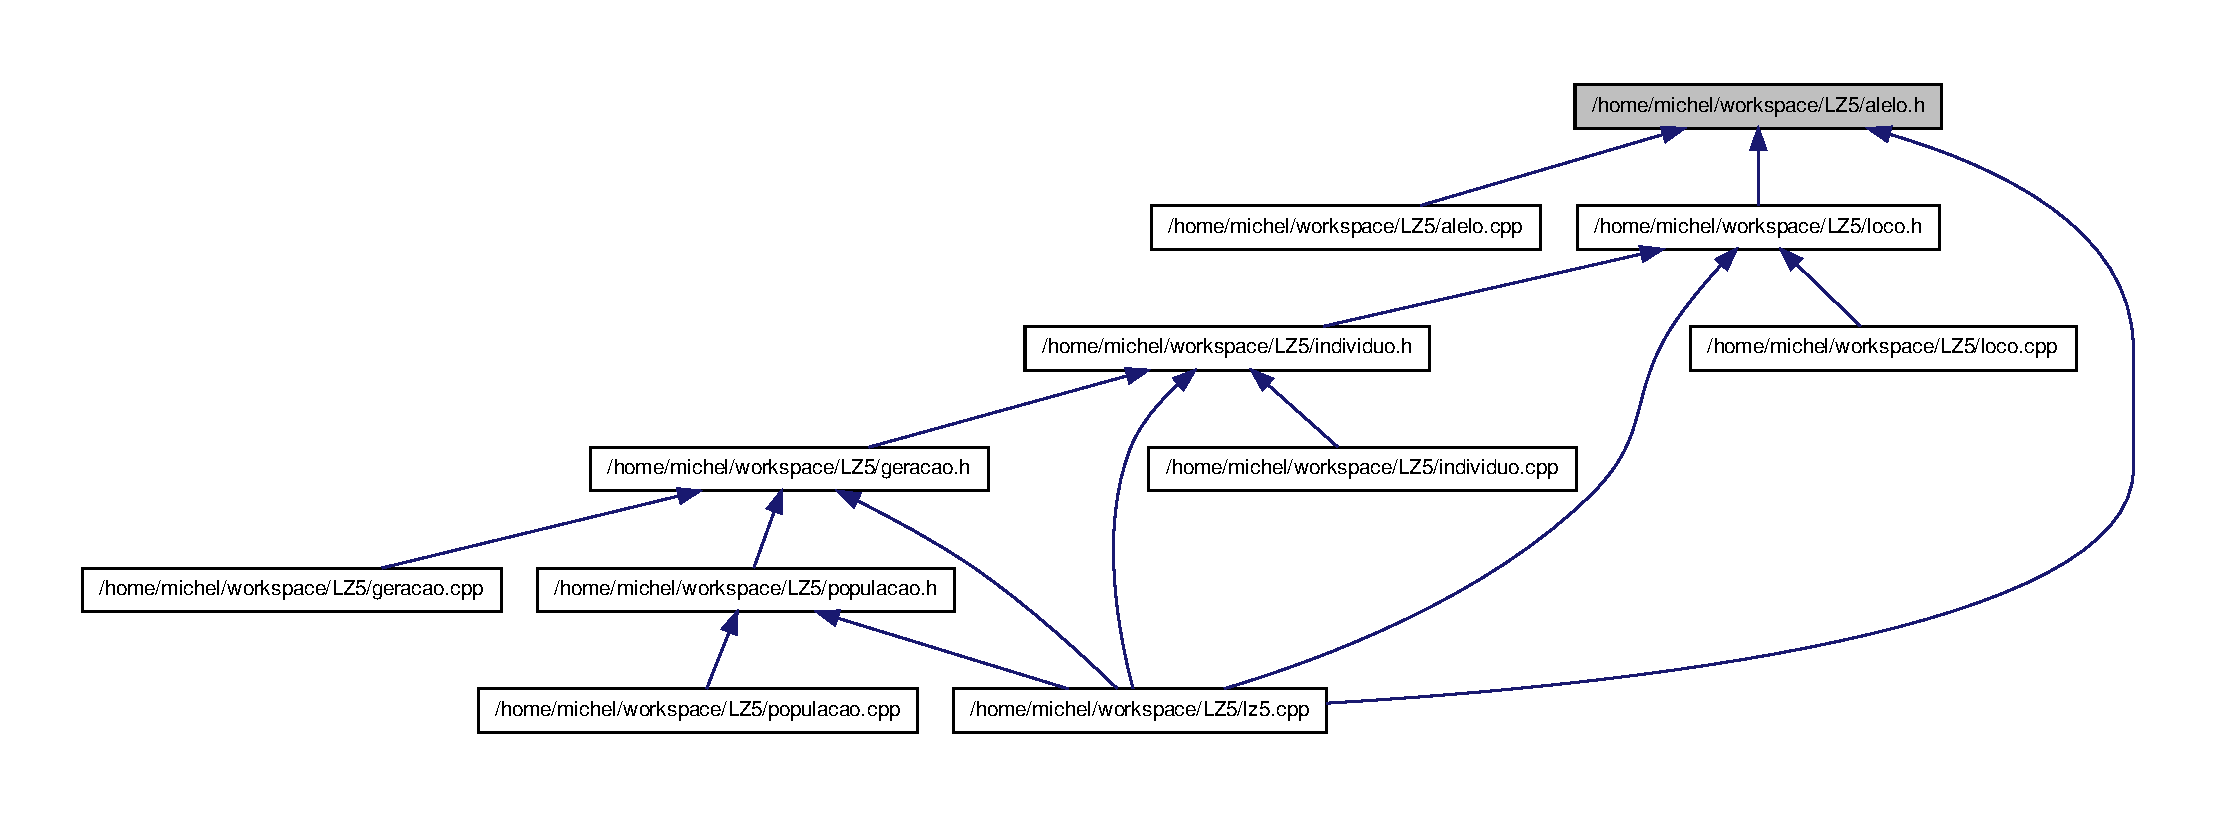
\includegraphics[width=350pt]{alelo_8h__dep__incl}
\end{center}
\end{figure}
\subsection*{\-Componentes}
\begin{DoxyCompactItemize}
\item 
class \hyperlink{class_alelo}{\-Alelo}
\begin{DoxyCompactList}\small\item\em \-Classe para criar um \hyperlink{class_alelo}{\-Alelo}. \end{DoxyCompactList}\item 
class \hyperlink{class_alelo_id}{\-Alelo\-Id}
\begin{DoxyCompactList}\small\item\em \-Classe derivada para criar um \hyperlink{class_alelo}{\-Alelo} com sua identificacao (\-I\-D). \end{DoxyCompactList}\end{DoxyCompactItemize}

\hypertarget{geracao_8cpp}{\section{\-Referência ao ficheiro /home/michel/workspace/\-L\-Z5/geracao.cpp}
\label{geracao_8cpp}\index{/home/michel/workspace/\-L\-Z5/geracao.\-cpp@{/home/michel/workspace/\-L\-Z5/geracao.\-cpp}}
}
{\ttfamily \#include \char`\"{}geracao.\-h\char`\"{}}\*
\-Diagrama de dependências de inclusão para geracao.\-cpp\-:\nopagebreak
\begin{figure}[H]
\begin{center}
\leavevmode
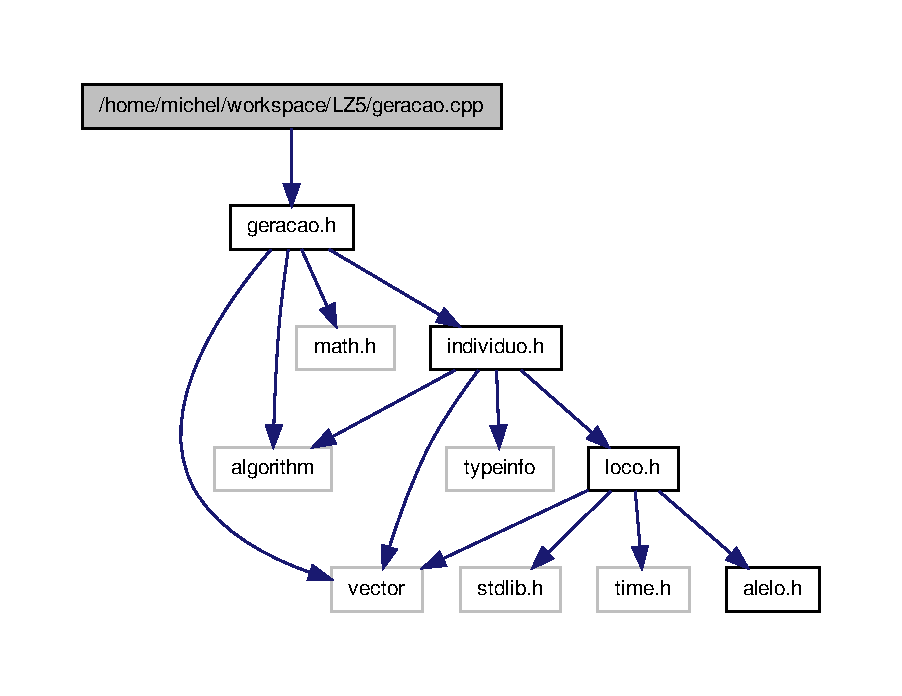
\includegraphics[width=350pt]{geracao_8cpp__incl}
\end{center}
\end{figure}

\hypertarget{geracao_8h}{\section{\-Referência ao ficheiro /home/michel/workspace/\-L\-Z5/geracao.h}
\label{geracao_8h}\index{/home/michel/workspace/\-L\-Z5/geracao.\-h@{/home/michel/workspace/\-L\-Z5/geracao.\-h}}
}
{\ttfamily \#include $<$vector$>$}\*
{\ttfamily \#include $<$algorithm$>$}\*
{\ttfamily \#include $<$math.\-h$>$}\*
{\ttfamily \#include \char`\"{}individuo.\-h\char`\"{}}\*
\-Diagrama de dependências de inclusão para geracao.\-h\-:\nopagebreak
\begin{figure}[H]
\begin{center}
\leavevmode
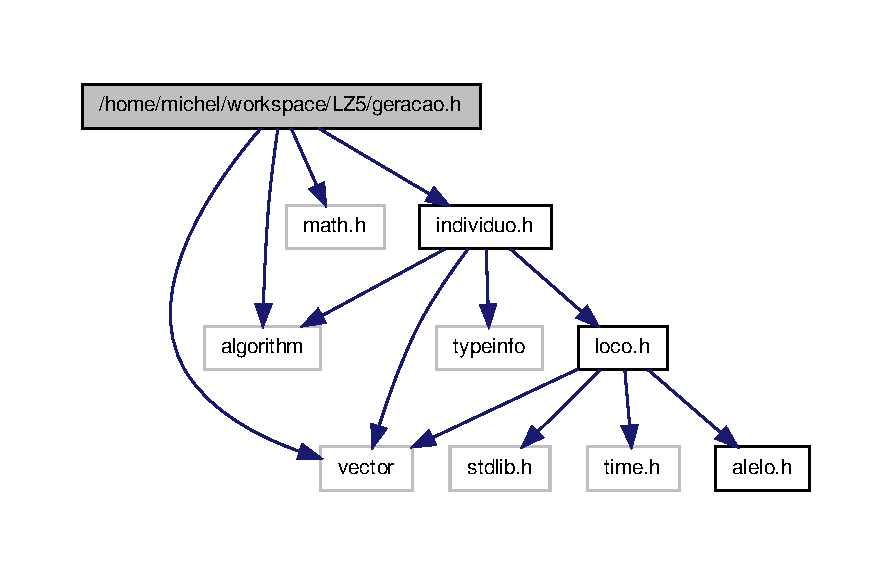
\includegraphics[width=350pt]{geracao_8h__incl}
\end{center}
\end{figure}
\-Este grafo mostra quais são os ficheiros que incluem directamente ou indirectamente este ficheiro\-:\nopagebreak
\begin{figure}[H]
\begin{center}
\leavevmode
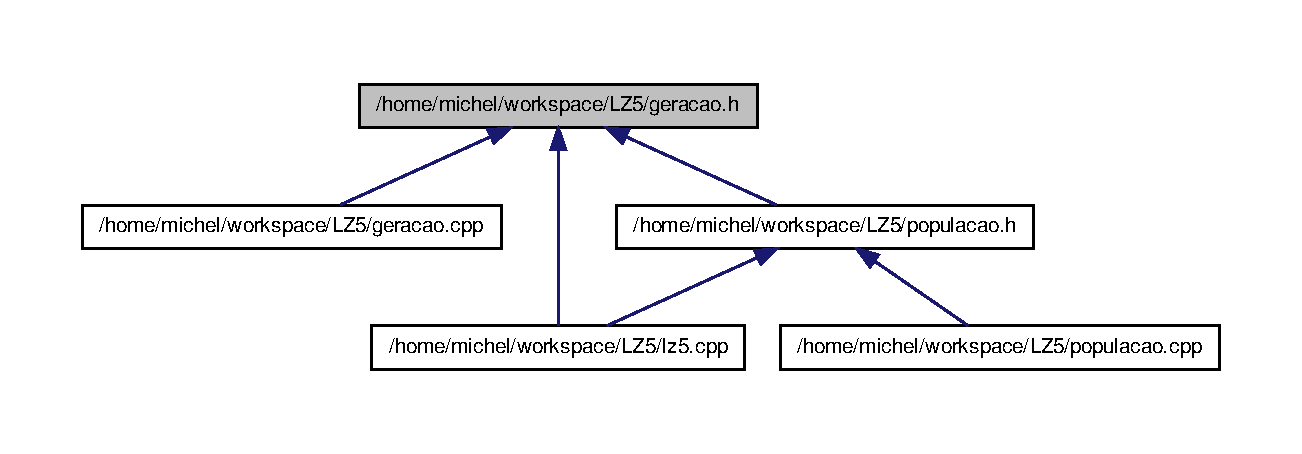
\includegraphics[width=350pt]{geracao_8h__dep__incl}
\end{center}
\end{figure}
\subsection*{\-Componentes}
\begin{DoxyCompactItemize}
\item 
class \hyperlink{class_geracao}{\-Geracao}
\begin{DoxyCompactList}\small\item\em \-Cria uma \hyperlink{class_geracao}{\-Geracao} que ira constituir uma populacao. \end{DoxyCompactList}\end{DoxyCompactItemize}

\hypertarget{individuo_8cpp}{\section{\-Referência ao ficheiro /home/michel/workspace/\-L\-Z5/individuo.cpp}
\label{individuo_8cpp}\index{/home/michel/workspace/\-L\-Z5/individuo.\-cpp@{/home/michel/workspace/\-L\-Z5/individuo.\-cpp}}
}
{\ttfamily \#include $<$vector$>$}\*
{\ttfamily \#include $<$stdlib.\-h$>$}\*
{\ttfamily \#include $<$time.\-h$>$}\*
{\ttfamily \#include $<$gsl/gsl\-\_\-rng.\-h$>$}\*
{\ttfamily \#include $<$gsl/gsl\-\_\-randist.\-h$>$}\*
{\ttfamily \#include $<$iostream$>$}\*
{\ttfamily \#include \char`\"{}individuo.\-h\char`\"{}}\*
\-Diagrama de dependências de inclusão para individuo.\-cpp\-:\nopagebreak
\begin{figure}[H]
\begin{center}
\leavevmode
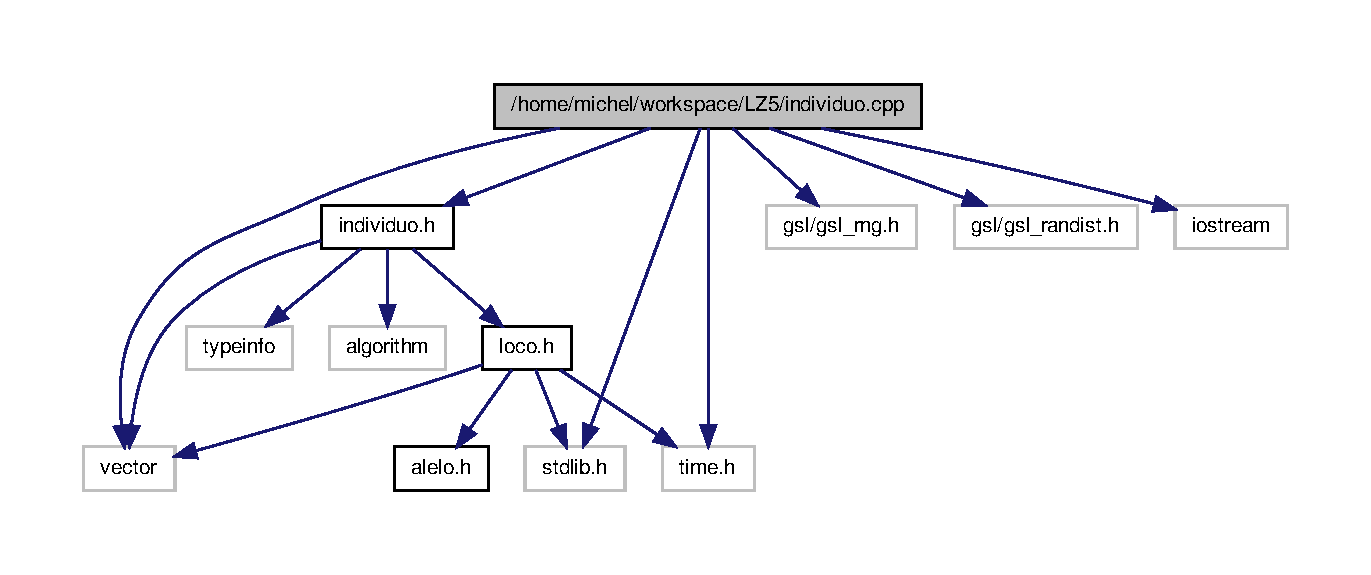
\includegraphics[width=350pt]{individuo_8cpp__incl}
\end{center}
\end{figure}
\subsection*{\-Variáveis}
\begin{DoxyCompactItemize}
\item 
gsl\-\_\-rng $\ast$ \hyperlink{individuo_8cpp_a726dba5c9e390fdbaf0e1f0a34045f2a}{p}
\end{DoxyCompactItemize}


\subsection{\-Documentação das variáveis}
\hypertarget{individuo_8cpp_a726dba5c9e390fdbaf0e1f0a34045f2a}{\index{individuo.\-cpp@{individuo.\-cpp}!p@{p}}
\index{p@{p}!individuo.cpp@{individuo.\-cpp}}
\subsubsection[{p}]{\setlength{\rightskip}{0pt plus 5cm}gsl\-\_\-rng$\ast$ {\bf p}}}\label{individuo_8cpp_a726dba5c9e390fdbaf0e1f0a34045f2a}

\hypertarget{individuo_8h}{\section{\-Referência ao ficheiro /home/michel/workspace/\-L\-Z5/individuo.h}
\label{individuo_8h}\index{/home/michel/workspace/\-L\-Z5/individuo.\-h@{/home/michel/workspace/\-L\-Z5/individuo.\-h}}
}
{\ttfamily \#include $<$vector$>$}\*
{\ttfamily \#include $<$typeinfo$>$}\*
{\ttfamily \#include $<$algorithm$>$}\*
{\ttfamily \#include \char`\"{}loco.\-h\char`\"{}}\*
\-Diagrama de dependências de inclusão para individuo.\-h\-:\nopagebreak
\begin{figure}[H]
\begin{center}
\leavevmode
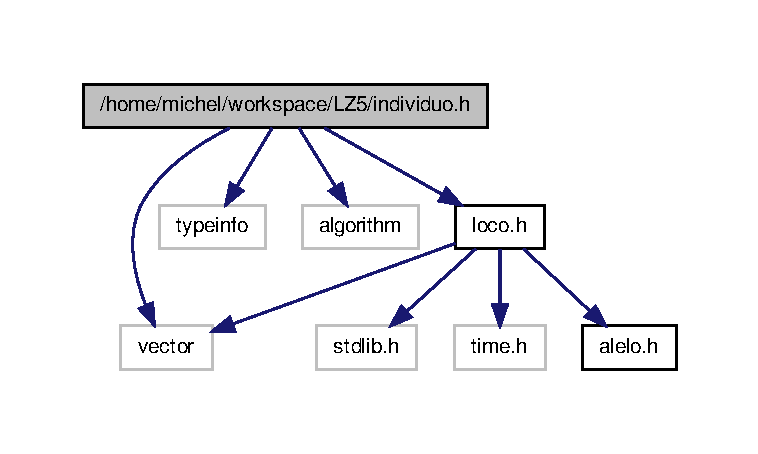
\includegraphics[width=350pt]{individuo_8h__incl}
\end{center}
\end{figure}
\-Este grafo mostra quais são os ficheiros que incluem directamente ou indirectamente este ficheiro\-:\nopagebreak
\begin{figure}[H]
\begin{center}
\leavevmode
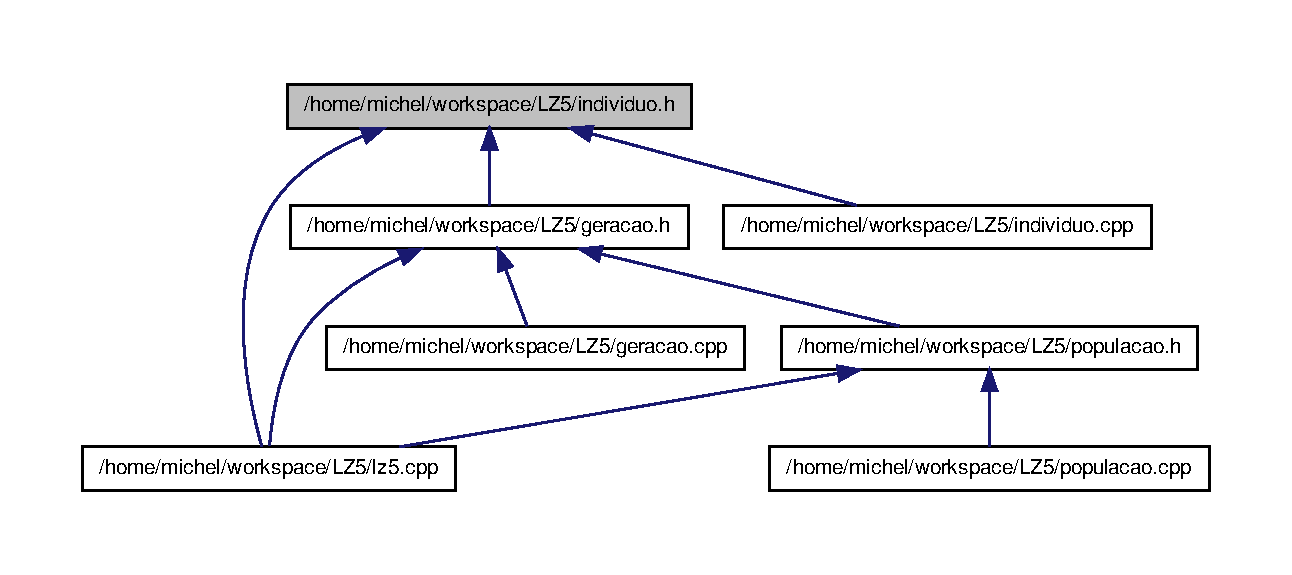
\includegraphics[width=350pt]{individuo_8h__dep__incl}
\end{center}
\end{figure}
\subsection*{\-Componentes}
\begin{DoxyCompactItemize}
\item 
class \hyperlink{class_individuo}{\-Individuo}
\begin{DoxyCompactList}\small\item\em \-Cria um genoma que constitui um individuo. \end{DoxyCompactList}\end{DoxyCompactItemize}

\hypertarget{loco_8cpp}{\section{\-Referência ao ficheiro /home/michel/workspace/\-L\-Z5/loco.cpp}
\label{loco_8cpp}\index{/home/michel/workspace/\-L\-Z5/loco.\-cpp@{/home/michel/workspace/\-L\-Z5/loco.\-cpp}}
}
{\ttfamily \#include $<$stdlib.\-h$>$}\*
{\ttfamily \#include $<$time.\-h$>$}\*
{\ttfamily \#include $<$cmath$>$}\*
{\ttfamily \#include \char`\"{}loco.\-h\char`\"{}}\*
\-Diagrama de dependências de inclusão para loco.\-cpp\-:\nopagebreak
\begin{figure}[H]
\begin{center}
\leavevmode
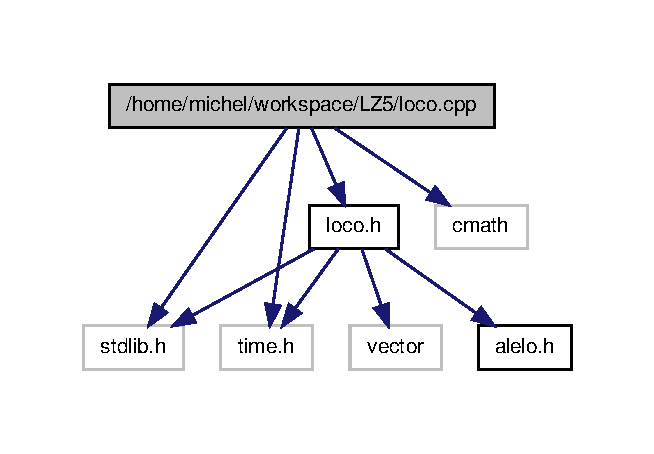
\includegraphics[width=314pt]{loco_8cpp__incl}
\end{center}
\end{figure}

\hypertarget{loco_8h}{\section{\-Referência ao ficheiro /home/michel/workspace/\-L\-Z5/loco.h}
\label{loco_8h}\index{/home/michel/workspace/\-L\-Z5/loco.\-h@{/home/michel/workspace/\-L\-Z5/loco.\-h}}
}
{\ttfamily \#include $<$stdlib.\-h$>$}\*
{\ttfamily \#include $<$time.\-h$>$}\*
{\ttfamily \#include $<$vector$>$}\*
{\ttfamily \#include \char`\"{}alelo.\-h\char`\"{}}\*
\-Diagrama de dependências de inclusão para loco.\-h\-:\nopagebreak
\begin{figure}[H]
\begin{center}
\leavevmode
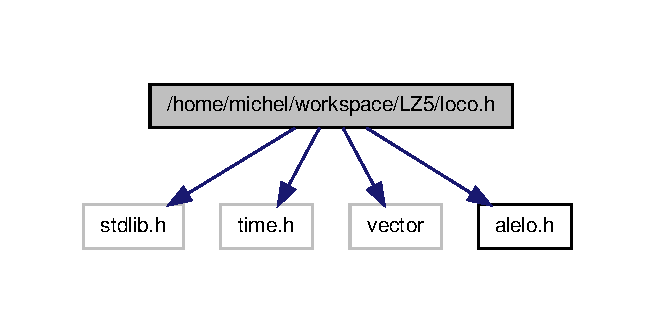
\includegraphics[width=314pt]{loco_8h__incl}
\end{center}
\end{figure}
\-Este grafo mostra quais são os ficheiros que incluem directamente ou indirectamente este ficheiro\-:\nopagebreak
\begin{figure}[H]
\begin{center}
\leavevmode
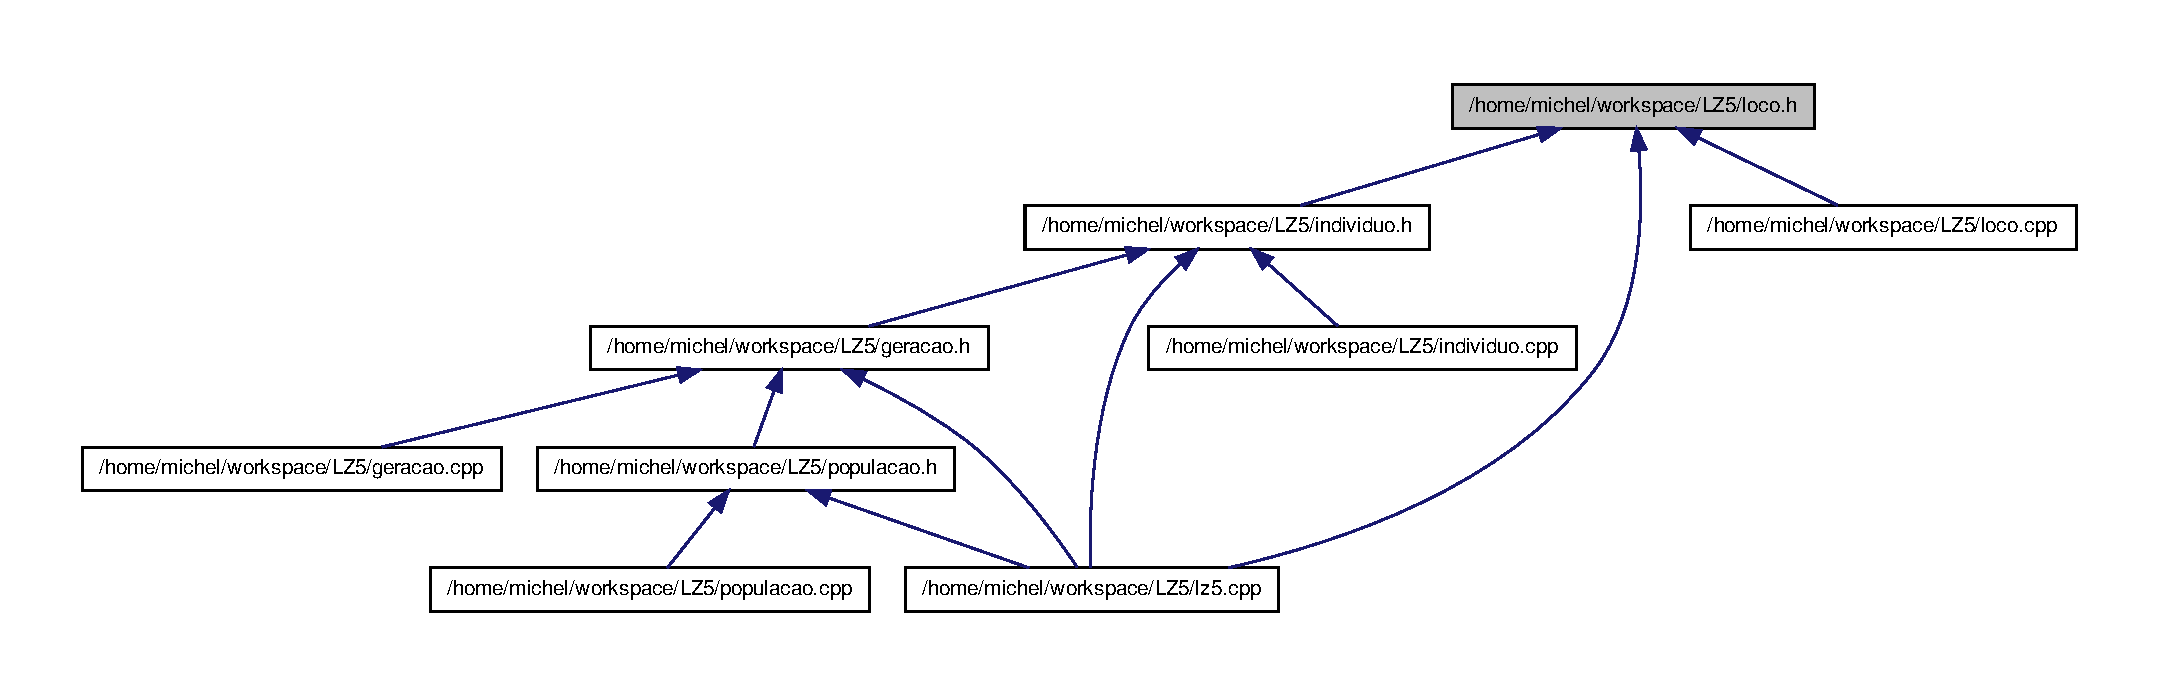
\includegraphics[width=350pt]{loco_8h__dep__incl}
\end{center}
\end{figure}
\subsection*{\-Componentes}
\begin{DoxyCompactItemize}
\item 
class \hyperlink{class_loco}{\-Loco}
\begin{DoxyCompactList}\small\item\em \-Classe para criar um \hyperlink{class_loco}{\-Loco} a partir de 2 \-Alelos. \end{DoxyCompactList}\end{DoxyCompactItemize}

\hypertarget{lz5_8cpp}{\section{\-Referência ao ficheiro /home/michel/workspace/\-L\-Z5/lz5.cpp}
\label{lz5_8cpp}\index{/home/michel/workspace/\-L\-Z5/lz5.\-cpp@{/home/michel/workspace/\-L\-Z5/lz5.\-cpp}}
}
{\ttfamily \#include $<$iostream$>$}\*
{\ttfamily \#include $<$vector$>$}\*
{\ttfamily \#include $<$typeinfo$>$}\*
{\ttfamily \#include $<$algorithm$>$}\*
{\ttfamily \#include $<$math.\-h$>$}\*
{\ttfamily \#include $<$gsl/gsl\-\_\-rng.\-h$>$}\*
{\ttfamily \#include $<$gsl/gsl\-\_\-randist.\-h$>$}\*
{\ttfamily \#include \char`\"{}alelo.\-h\char`\"{}}\*
{\ttfamily \#include \char`\"{}loco.\-h\char`\"{}}\*
{\ttfamily \#include \char`\"{}individuo.\-h\char`\"{}}\*
{\ttfamily \#include \char`\"{}geracao.\-h\char`\"{}}\*
{\ttfamily \#include \char`\"{}populacao.\-h\char`\"{}}\*
\-Diagrama de dependências de inclusão para lz5.\-cpp\-:\nopagebreak
\begin{figure}[H]
\begin{center}
\leavevmode
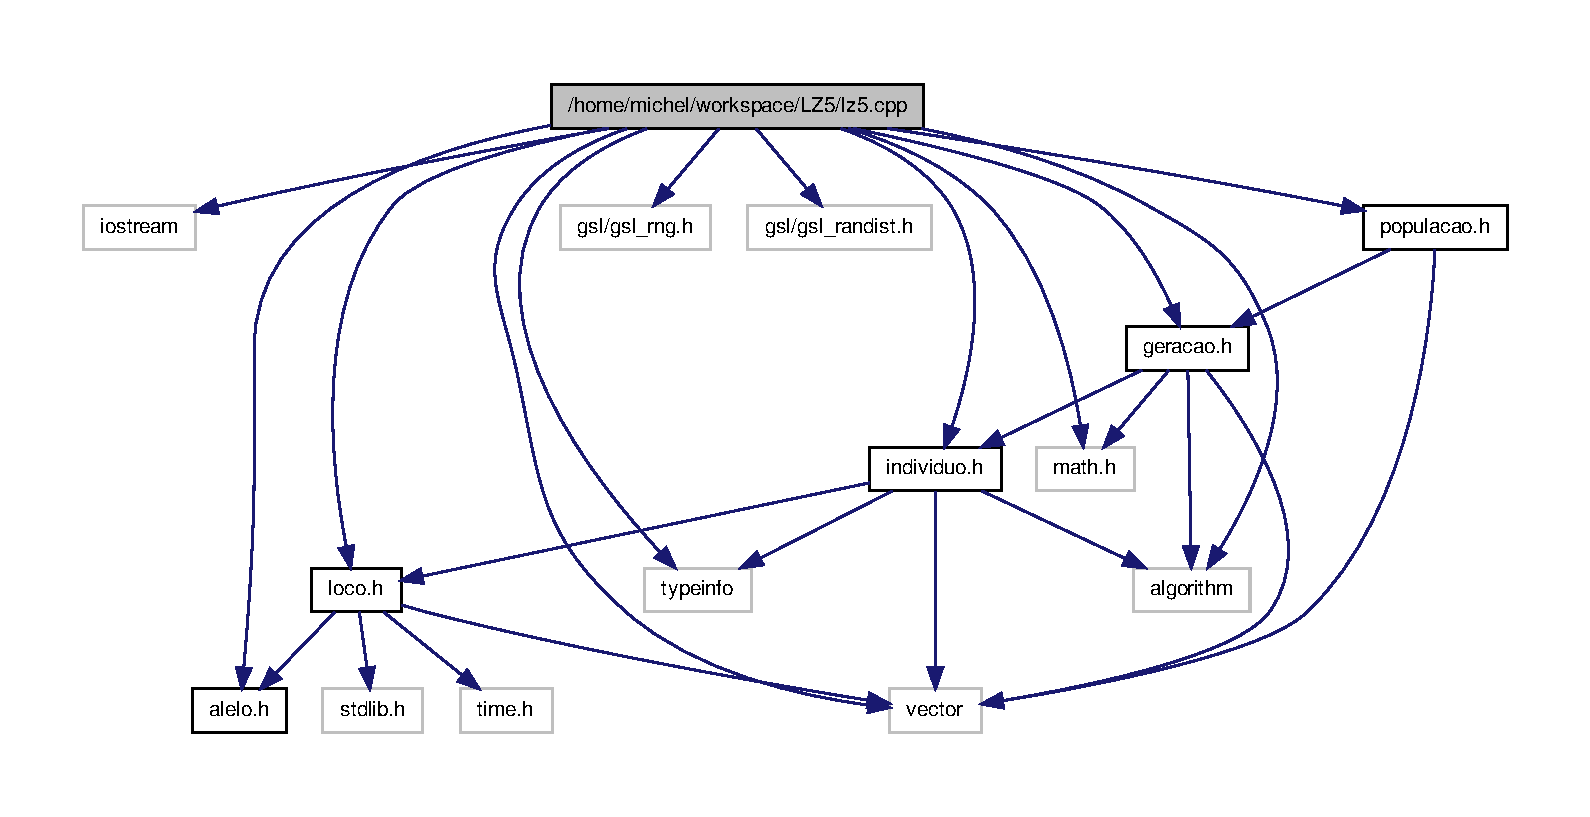
\includegraphics[width=350pt]{lz5_8cpp__incl}
\end{center}
\end{figure}
\subsection*{\-Funções}
\begin{DoxyCompactItemize}
\item 
int \hyperlink{lz5_8cpp_ae66f6b31b5ad750f1fe042a706a4e3d4}{main} ()
\end{DoxyCompactItemize}
\subsection*{\-Variáveis}
\begin{DoxyCompactItemize}
\item 
gsl\-\_\-rng $\ast$ \hyperlink{lz5_8cpp_a726dba5c9e390fdbaf0e1f0a34045f2a}{p} = gsl\-\_\-rng\-\_\-alloc(gsl\-\_\-rng\-\_\-mt19937)
\end{DoxyCompactItemize}


\subsection{\-Documentação das funções}
\hypertarget{lz5_8cpp_ae66f6b31b5ad750f1fe042a706a4e3d4}{\index{lz5.\-cpp@{lz5.\-cpp}!main@{main}}
\index{main@{main}!lz5.cpp@{lz5.\-cpp}}
\subsubsection[{main}]{\setlength{\rightskip}{0pt plus 5cm}int {\bf main} (
\begin{DoxyParamCaption}
{}
\end{DoxyParamCaption}
)}}\label{lz5_8cpp_ae66f6b31b5ad750f1fe042a706a4e3d4}


\-Grafo de chamadas desta função\-:\nopagebreak
\begin{figure}[H]
\begin{center}
\leavevmode
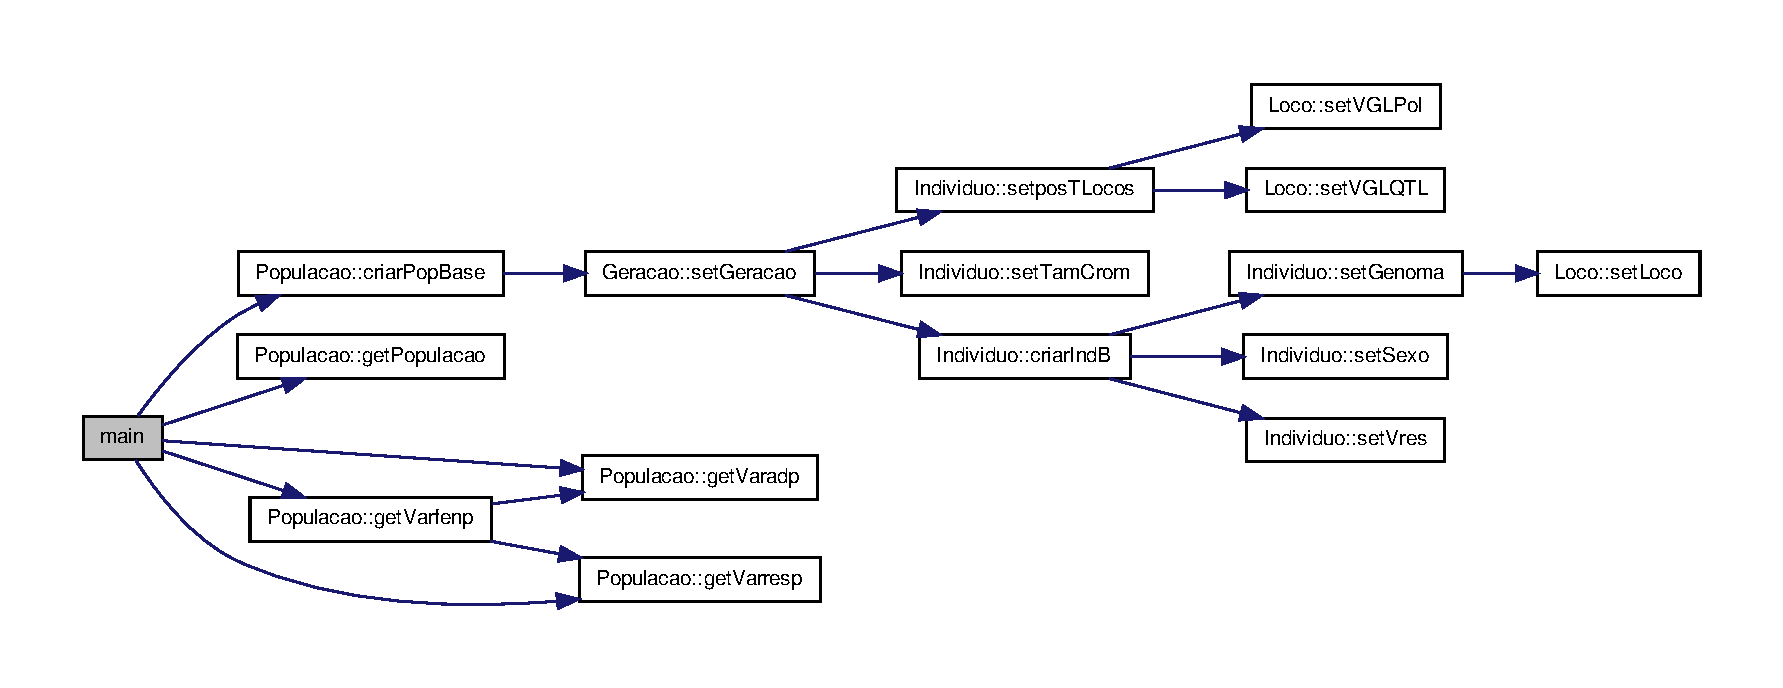
\includegraphics[width=350pt]{lz5_8cpp_ae66f6b31b5ad750f1fe042a706a4e3d4_cgraph}
\end{center}
\end{figure}




\subsection{\-Documentação das variáveis}
\hypertarget{lz5_8cpp_a726dba5c9e390fdbaf0e1f0a34045f2a}{\index{lz5.\-cpp@{lz5.\-cpp}!p@{p}}
\index{p@{p}!lz5.cpp@{lz5.\-cpp}}
\subsubsection[{p}]{\setlength{\rightskip}{0pt plus 5cm}gsl\-\_\-rng$\ast$ {\bf p} = gsl\-\_\-rng\-\_\-alloc(gsl\-\_\-rng\-\_\-mt19937)}}\label{lz5_8cpp_a726dba5c9e390fdbaf0e1f0a34045f2a}

\hypertarget{populacao_8cpp}{\section{\-Referência ao ficheiro /home/michel/workspace/\-L\-Z5/populacao.cpp}
\label{populacao_8cpp}\index{/home/michel/workspace/\-L\-Z5/populacao.\-cpp@{/home/michel/workspace/\-L\-Z5/populacao.\-cpp}}
}
{\ttfamily \#include \char`\"{}populacao.\-h\char`\"{}}\*
\-Diagrama de dependências de inclusão para populacao.\-cpp\-:\nopagebreak
\begin{figure}[H]
\begin{center}
\leavevmode
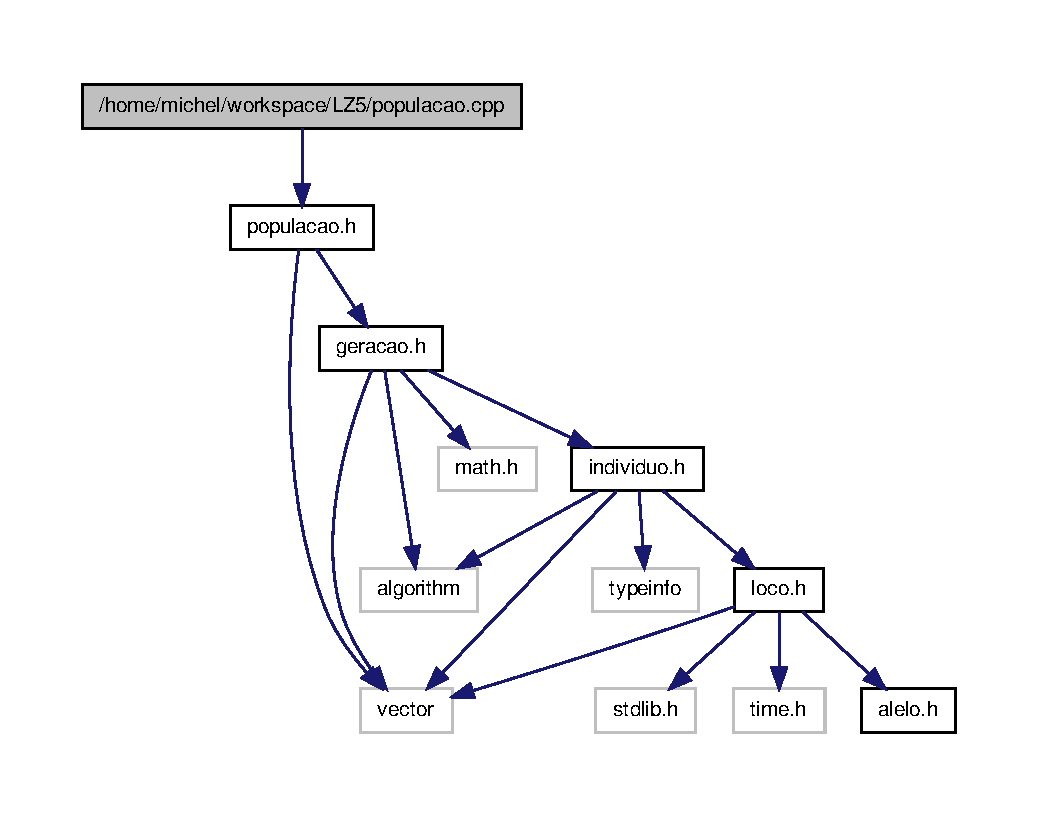
\includegraphics[width=350pt]{populacao_8cpp__incl}
\end{center}
\end{figure}

\hypertarget{populacao_8h}{\section{\-Referência ao ficheiro /home/michel/workspace/\-L\-Z5/populacao.h}
\label{populacao_8h}\index{/home/michel/workspace/\-L\-Z5/populacao.\-h@{/home/michel/workspace/\-L\-Z5/populacao.\-h}}
}
{\ttfamily \#include $<$vector$>$}\*
{\ttfamily \#include \char`\"{}geracao.\-h\char`\"{}}\*
\-Diagrama de dependências de inclusão para populacao.\-h\-:\nopagebreak
\begin{figure}[H]
\begin{center}
\leavevmode
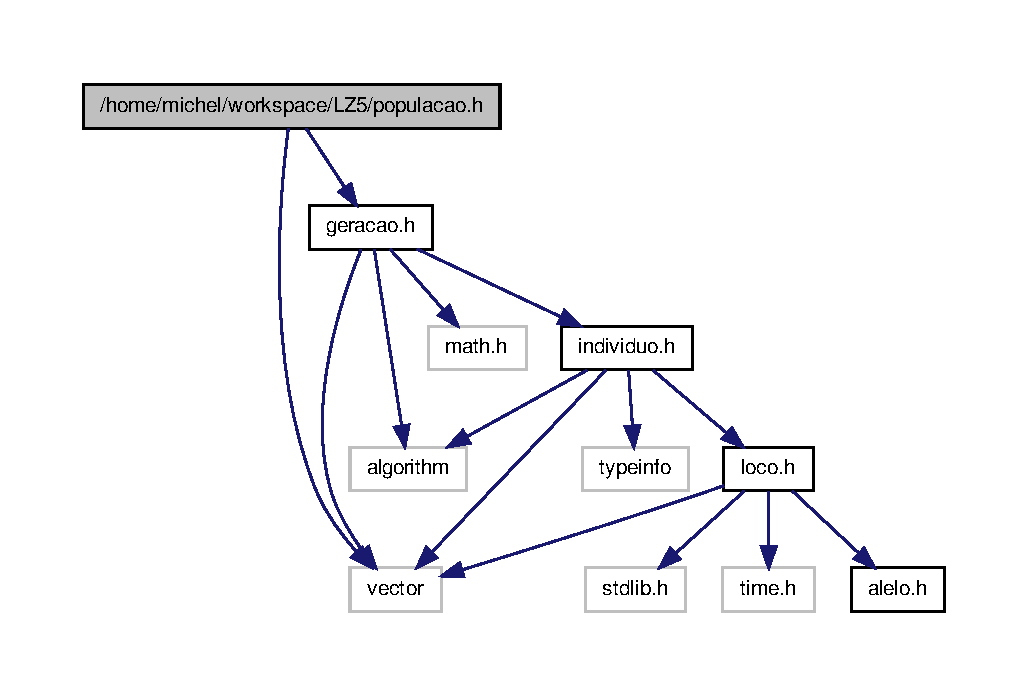
\includegraphics[width=350pt]{populacao_8h__incl}
\end{center}
\end{figure}
\-Este grafo mostra quais são os ficheiros que incluem directamente ou indirectamente este ficheiro\-:\nopagebreak
\begin{figure}[H]
\begin{center}
\leavevmode
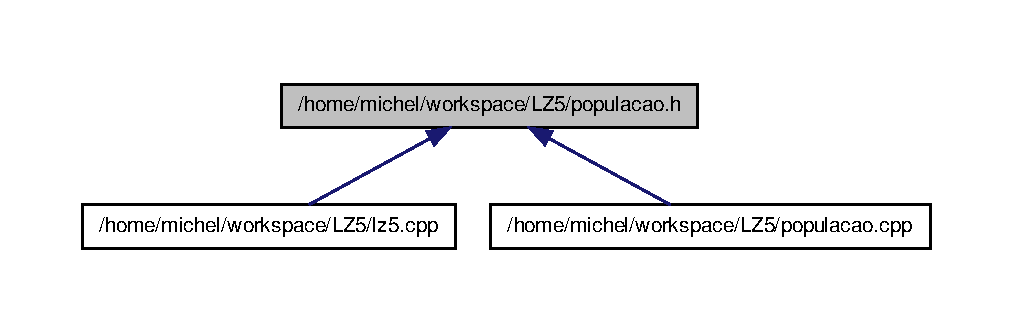
\includegraphics[width=350pt]{populacao_8h__dep__incl}
\end{center}
\end{figure}
\subsection*{\-Componentes}
\begin{DoxyCompactItemize}
\item 
class \hyperlink{class_populacao}{\-Populacao}
\begin{DoxyCompactList}\small\item\em \-Cria uma \hyperlink{class_populacao}{\-Populacao}, constituida de diversas \-Geracoes. \end{DoxyCompactList}\end{DoxyCompactItemize}

\printindex
\end{document}
